\def\figpath{tex/5_Differenzverstaerker/pictures}
\graphicspath{{tex/5_Differenzverstaerker/pictures/}}

\chapter{Differenzverstärker}
In Kapitel 5 werden die Eigenschaften einer einfachen und einer erweiterten Differenzverstärkerschaltung untersucht.

\section{Einfacher Differenzverstärker}
Abb. \ref{} zeigt das Ersatzschaltbild eines einfachen Differenzverstärkers mit einem einzigen Ausgang. 

\begin{figure}[H]
	\centering
	\def\svgwidth{0.7\textwidth}
	\input{\figpath/DiffVerstärker.pdf_tex}
	\caption{Einfacher Differenzverstärker} 
	\label{fig_Kap5_01:ESBDiffVerst} 
\end{figure}

\subsection{Dimensionierung der Kollektorwiderstände $R_C$}

Im ersten Schritt müssen die Kollektorwiderstände dermaßen dimensioniert werden, so dass die Kollektorpotentiale, im Arbeitspunkt $U_P = U_N = \SI{0}{\volt}$, auf \SI{7.5}{\volt} liegen. Die Emitterwiderstände sollen \SI{33}{\ohm} betragen.

Der Strom der Stromquelle von \SI{10}{\milli \ampere} teilt sich gleichmäßig auf die Beiden Kollektorströme ($I_{c1} = I_{c2} = I_c$ auf (Basisströme werden gerechtfertigterweise vernachlässigt). Der Strom durch die Kollektorwiderstände beträgt also jeweils \SI{5}{\milli \ampere} und an den beiden Widerständen soll \SI{7.5}{\volt} abfallen. Dies liefert über das ohmsche Gesetz den gesuchten Widerstandswert:

\begin{equation}
    V_c = \SI{7.5}{\volt} = \SI{15}{\volt} - R_c I_c \rightarrow Rc = \frac{\SI{7.5}{\volt} - \SI{15}{\volt}}{- I_c} = \SI{1.5}{\kilo \ohm}
\end{equation}

\subsection{Kleinsignal-Spannungsverstärkung $A_{ed}$}
Im nächsten Schritt soll die Kleinsignal-Spannungsverstärkung nach

\begin{equation}
    A_{ed} = \frac{u_A}{u_P - u_N}
\end{equation}

für die Fälle $R_E = \SI{0}{\ohm}$ und $R_E = \SI{33}{\ohm}$berechnet und simuliert werden. Dafür wird zunächst das KSESB betrachtet, siehe Abb. \ref{fig_Kap5_02:ESBDiffVerstKSBES}.

\begin{figure}[H]
	\centering
	\def\svgwidth{0.9\textwidth}
	\input{\figpath/DiffVerstärker_1_KSESB.pdf_tex}
	\caption{Einfacher Differenzverstärker KSESB} 
	\label{fig_Kap5_02:ESBDiffVerstKSBES} 
\end{figure}

Des Weiteren soll es sich hier um eine schiefsymmetrische Aussteuerung handeln, sprich

\begin{equation}
    u_P = -u_N = u_E
\end{equation}

\begin{equation}
    \label{Gln_I}
    u_P = i{B,1} ( \frac{B}{S} + R_E\cdot (B + 1) ) + R_i \cdot (B+1)(i{B,1} + i{B,2}) = u_E
\end{equation}

\begin{equation}
    \label{Gln_II}
    u_N = i{B,2} ( \frac{B}{S} + R_E\cdot (B + 1) ) + R_i \cdot (B+1)(i{B,1} + i{B,2}) = -u_E
\end{equation}

Subtrahiert man beide Gleichungen voneinander, erhält man

\begin{equation}
    i_{B,1} \cdot \left( -\frac{B}{S} - R_E(B+1) - 2R_i(B+1) \right) = i_{B,2} \cdot \left( +\frac{B}{S} + R_E(B+1) + 2R_i(B+1) \right)
\end{equation}

\begin{equation}
    \label{current}
    i_{B,1} = -i_{B,2}
\end{equation}

Für die Ausgangsspannung gilt

\begin{equation}
    u_a = -R_C B i_{B,2} = R_C B i_{B,1}
\end{equation}

Legt man eine Maschen von $u_P$ bis $u_N$ gelangt man zum Zusammenhang

\begin{equation}
    u_P = \left( \frac{B}{S} + R_E(B+1) \right) (i_{B,1} - i_{B,2} ) + u_N, 
\end{equation}

woraus folgt dass mit Glng. \ref{current} gilt

\begin{equation}
    u_P - u_N = 2i_{B,1} \left( \frac{B}{S} + R_E(B+1) \right)
\end{equation}

Setzt man dies in Glng. 5.2 ein, so erhält man für die Differenzverstärkung

\begin{equation}
    A_{ed} = \frac{R_C B i_{B,1}}{2i_{B,1} \left( \frac{B}{S} + R_E(B+1) \right)} = \frac{R_C S}{2\left( 1 + R_E S(1+\frac{1}{B}) \right)} \approx \frac{R_C S}{2\left( 1 + R_E S \right)}
\end{equation}

Für die in Tab. \ref{tab_Kap5_01:Bauteilwerte} angeführten Parameter gilt lässt sich die Differenzverstärkung berechnen.

\begin{table}[H]
\centering
\begin{tabular}{|c|c|} \hline
Benennung & Größe \\ \hline
$R_C$ & \SI{1500}{\ohm} \\ \hline
$I_{C,0}$ & \SI{5}{\milli\ampere} \\ \hline
$B$ & 290 \\ \hline
$U_T$ & \SI{25,9}{\milli\volt} \\ \hline
\end{tabular}
\caption{Parameter für Berechnung und Simulation}
\label{tab_Kap5_01:Bauteilwerte} 
\end{table}

Für einen Emitterwiderstand von $R_E = \SI{33}{\ohm}$ gilt somit

\begin{equation}
    A_{ed} = \frac{R_C S}{2\left( 1 + R_E S(1+\frac{1}{B}) \right)} = \frac{\SI{1500}{\ohm}\cdot\SI{0,2}{\ampere\per\volt}}{2(1+\SI{33}{\ohm} \cdot \SI{0,2}{\ampere\per\volt} (1 + \frac{1}{290}) )} = 19.68 \hat{=} 25.88\text{dB} .
\end{equation}

Für einen Emitterwiderstand von $R_E = \SI{0}{\ohm}$ gilt dagegen

\begin{equation}
    A_{ed} = \frac{R_C S}{2} =  \frac{\SI{1500}{\ohm}\cdot\SI{0,2}{\ampere\per\volt}}{2} = 150 \hat{=} 43.5\text{dB} .
\end{equation}

Nun wird die Kleinsignalverstärkung simuliert, siehe Abb. \ref{fig_Kap5_03:SpiceSchematic}.

\begin{figure}[H]
    \centering
    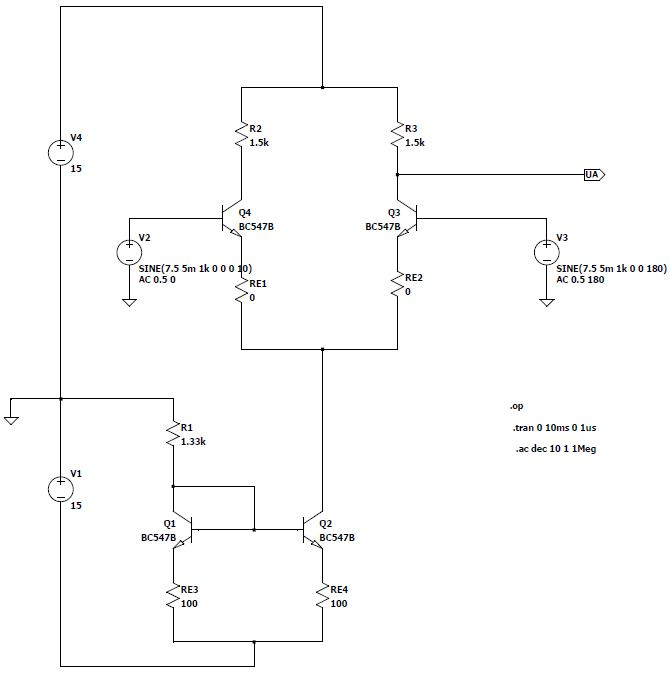
\includegraphics[width = 0.6\textwidth]{\figpath/einfachDiff.jpg}
    \caption{Einfacher Stromspiegel in LTSpice}
    \label{fig_Kap5_03:SpiceSchematic}
\end{figure}

Mit einer AC-Analyse kann das Bode-Diagramm und daraus die Verstärkung abgelesen werden. Mit $R_E = \SI{0}{\ohm}$ wird eine Verstärkung von 

\begin{equation}
    A_{ed} = 41.17\text{dB} \hat{=} 114.4
\end{equation}

simuliert. Mit $R_E = \SI{33}{\ohm}$ wird hingegen eine Verstärkung von 

\begin{equation}
    A_{ed} = 25.5\text{dB} \hat{=} 18.8
\end{equation}

erreicht. Die Verstärkung bei $R_E = \SI{0}{\ohm}$ weicht doch beträchtlich vom berechneten Wert ab.

\begin{figure}[H]
	\centering \small
	\scalebox{0.9}{% This file was created by matlab2tikz.
%
\definecolor{mycolor1}{rgb}{0.00000,0.44700,0.74100}%
\definecolor{mycolor2}{rgb}{0.85000,0.32500,0.09800}%
%
\begin{tikzpicture}

\begin{axis}[%
width=4.521in,
height=3.566in,
at={(0.758in,0.481in)},
scale only axis,
xmode=log,
xmin=1,
xmax=100000000,
xminorticks=true,
xlabel style={font=\color{white!15!black}},
xlabel={$f \text{ in } \text{Hz}$},
ymin=10,
ymax=45,
ylabel style={font=\color{white!15!black}},
ylabel={$A_{ed} \text{ in } \text{dB}$},
axis background/.style={fill=white},
title style={font=\bfseries},
title={$A_{ed}$},
xmajorgrids,
xminorgrids,
ymajorgrids,
legend style={at={(0.03,0.03)}, anchor=south west, legend cell align=left, align=left, draw=white!15!black}
]
\addplot [color=mycolor1]
  table[row sep=crcr]{%
1	41.1675597085499\\
1.25892541179417	41.1675597085499\\
1.58489319246111	41.1675597085499\\
1.99526231496888	41.1675597085499\\
2.51188643150958	41.1675597085499\\
3.16227766016838	41.1675597085499\\
3.98107170553497	41.1675597085499\\
5.01187233627272	41.1675597085498\\
6.30957344480194	41.1675597085497\\
7.94328234724282	41.1675597085496\\
10	41.1675597085494\\
12.5892541179417	41.1675597085491\\
15.8489319246111	41.1675597085486\\
19.9526231496888	41.1675597085478\\
25.1188643150958	41.1675597085466\\
31.6227766016838	41.1675597085447\\
39.8107170553498	41.1675597085416\\
50.1187233627273	41.1675597085367\\
63.0957344480194	41.167559708529\\
79.4328234724283	41.1675597085168\\
100	41.1675597084974\\
125.892541179417	41.1675597084666\\
158.489319246112	41.1675597084179\\
199.526231496888	41.1675597083407\\
251.188643150958	41.1675597082183\\
316.227766016838	41.1675597080244\\
398.107170553498	41.1675597077169\\
501.187233627273	41.1675597072297\\
630.957344480194	41.1675597064575\\
794.328234724283	41.1675597052337\\
1000	41.1675597032941\\
1258.92541179417	41.16755970022\\
1584.89319246112	41.1675596953478\\
1995.26231496888	41.167559687626\\
2511.88643150959	41.1675596753877\\
3162.27766016839	41.1675596559913\\
3981.07170553498	41.1675596252502\\
5011.87233627273	41.1675595765287\\
6309.57344480195	41.1675594993104\\
7943.28234724283	41.1675593769276\\
10000	41.167559182964\\
12589.2541179417	41.1675588755524\\
15848.9319246112	41.1675583883378\\
19952.6231496889	41.1675576161549\\
25118.8643150959	41.1675563923278\\
31622.7766016839	41.1675544526933\\
39810.7170553498	41.1675513785814\\
50118.7233627274	41.1675465064469\\
63095.7344480195	41.1675387846453\\
79432.8234724284	41.1675265464426\\
100000	41.1675071502689\\
125892.541179417	41.1674764095824\\
158489.319246112	41.1674276893225\\
199526.231496889	41.1673504740319\\
251188.643150959	41.1672280988505\\
316227.766016839	41.1670341543093\\
398107.170553499	41.166726790635\\
501187.233627274	41.1662396965157\\
630957.344480196	41.1654678160529\\
794328.234724285	41.1642447484103\\
1000000	41.1623070208594\\
1258925.41179417	41.1592376964086\\
1584893.19246112	41.1543775761543\\
1995262.31496889	41.1466859086149\\
2511886.43150959	41.1345232234583\\
3162277.66016839	41.1153160457674\\
3981071.70553499	41.0850473530381\\
5011872.33627275	41.0375019329754\\
6309573.44480196	40.9631958938044\\
7943282.34724285	40.8479680048281\\
10000000	40.6713734757856\\
12589254.1179417	40.4053899925528\\
15848931.9246112	40.0145448431442\\
19952623.1496889	39.4590867279285\\
25118864.3150959	38.7023186825246\\
31622776.6016839	37.7206902592622\\
39810717.0553499	36.5118028909646\\
50118723.3627275	35.0950901786693\\
63095734.4480196	33.5046166915506\\
79432823.4724286	31.7787008679182\\
100000000	29.9515824393383\\
};
\addlegendentry{$R_E = \SI{0}{\ohm}$}

\addplot [color=mycolor2]
  table[row sep=crcr]{%
1	25.5228956217106\\
1.25892541179417	25.5228956217106\\
1.58489319246111	25.5228956217106\\
1.99526231496888	25.5228956217106\\
2.51188643150958	25.5228956217106\\
3.16227766016838	25.5228956217106\\
3.98107170553497	25.5228956217105\\
5.01187233627272	25.5228956217104\\
6.30957344480194	25.5228956217103\\
7.94328234724282	25.5228956217102\\
10	25.52289562171\\
12.5892541179417	25.5228956217097\\
15.8489319246111	25.5228956217091\\
19.9526231496888	25.5228956217083\\
25.1188643150958	25.522895621707\\
31.6227766016838	25.5228956217053\\
39.8107170553498	25.522895621702\\
50.1187233627273	25.5228956216969\\
63.0957344480194	25.5228956216888\\
79.4328234724283	25.5228956216764\\
100	25.5228956216565\\
125.892541179417	25.5228956216246\\
158.489319246112	25.5228956215747\\
199.526231496888	25.522895621495\\
251.188643150958	25.5228956213689\\
316.227766016838	25.5228956211692\\
398.107170553498	25.5228956208526\\
501.187233627273	25.5228956203507\\
630.957344480194	25.5228956195553\\
794.328234724283	25.5228956182946\\
1000	25.5228956162967\\
1258.92541179417	25.5228956131303\\
1584.89319246112	25.5228956081119\\
1995.26231496888	25.522895600158\\
2511.88643150959	25.5228955875521\\
3162.27766016839	25.522895567573\\
3981.07170553498	25.5228955359085\\
5011.87233627273	25.5228954857234\\
6309.57344480195	25.5228954061853\\
7943.28234724283	25.5228952801263\\
10000	25.5228950803359\\
12589.2541179417	25.5228947636896\\
15848.9319246112	25.5228942618392\\
19952.6231496889	25.5228934664598\\
25118.8643150959	25.5228922058687\\
31622.7766016839	25.5228902079673\\
39810.7170553498	25.5228870415087\\
50118.7233627274	25.5228820230149\\
63095.7344480195	25.5228740692496\\
79432.8234724284	25.5228614634109\\
100000	25.5228414845765\\
125892.541179417	25.5228098204432\\
158489.319246112	25.5227596366393\\
199526.231496889	25.522680101839\\
251188.643150959	25.5225540506117\\
316227.766016839	25.5223542802543\\
398107.170553499	25.5220376840981\\
501187.233627274	25.521535959526\\
630957.344480196	25.5207408964931\\
794328.234724285	25.5194810998442\\
1000000	25.5174851930922\\
1258925.41179417	25.5143237419672\\
1584893.19246112	25.5093178141362\\
1995262.31496889	25.50139556614\\
2511886.43150959	25.4888687067873\\
3162277.66016839	25.4690875162491\\
3981071.70553499	25.4379169103328\\
5011872.33627275	25.388961299833\\
6309573.44480196	25.3124669298499\\
7943282.34724285	25.1938817442867\\
10000000	25.0122223881563\\
12589254.1179417	24.7387772969232\\
15848931.9246112	24.3372786481545\\
19952623.1496889	23.7671643138976\\
25118864.3150959	22.9909584755781\\
31622776.6016839	21.98418128594\\
39810717.0553499	20.7428012574352\\
50118723.3627275	19.2831242864075\\
63095734.4480196	17.633952334075\\
79432823.4724286	15.82615136349\\
100000000	13.8853882468763\\
};
\addlegendentry{$R_E = \SI{33}{\ohm}$}

\end{axis}
\end{tikzpicture}%}
	\caption{Bodediagramm der Differenzverstärkung}
	\label{fig_Kap5_04:Bode}
\end{figure}

\subsection{Gleichtaktverstärkung $A_{gl}$}
Für die Gleichtaktaussteuerung wird eine symmetrische Aussteuerung mit Gleichtaktspannung $U_{gl}$ angenommen, 

\begin{equation}
    u_P = u_N = u_{gl} \quad \Rightarrow \quad u_{gl} = \frac{u_P + u_N}{2} .
\end{equation}

Womit sich gleiche Basisströme einstellen,

\begin{equation}
    i_{B,1} = i_{B,2} = i_{B} .
\end{equation}

Addiert man nun \ref{Gln_I} und \ref{Gln_II} erhält man

\begin{equation}
    u_P + u_N = 2 i_B \cdot \left( \frac{B}{S} + (R_E + 2 \cdot R_i)(B+1) \right) .
\end{equation}

Somit erhält man für die Gleichtaktverstärkung

\begin{equation}
    A_{gl} = \frac{2 \cdot u_a}{u_P + u_N} = -\frac{2BR_Ci_B}{2 i_B \cdot \left( \frac{B}{S} + (R_E + 2 \cdot R_i)(B+1) \right)} = - \frac{R_C}{\frac{1}{S} + (R_E + 2 \cdot R_i)(1+\frac{1}{B})} \approx -\frac{R_C}{R_E + 2R_i}
\end{equation}

Für die Berechnung wird nun lt. Abb. \ref{fig_Kap4_05:Ri} ein Widerstand von $R_i = \SI{250}{\kilo\ohm}$ angenommen (extrapolierter Wert bei einer Ausgangsspannung von $\SI{21,8}{\volt}$, hier wurde die Ausgangsspannung am Stromspiegel im Arbeitspunkt ermittelt). Im Vergleich dazu ist der gewählte Emitterwiderstand äußerst niedrig, womit sich die Gleichtaktverstärkung folgendermaßen berechnet, 

\begin{equation}
    A_{gl} \approx -\frac{R_C}{2R_i} = -\frac{\SI{1500}{\ohm}}{\SI{500}{\kilo\ohm}} = 0.003 \hat{=} -50.5 \text{dB} .
\end{equation}

Lt. Simulation ergibt sich ein Wert von 

\begin{equation}
    A_{gl} =-52.1 \text{dB} \hat{=} 0.0025 .
\end{equation}

\begin{figure}[H]
	\centering \small
	\scalebox{0.9}{% This file was created by matlab2tikz.
%
\definecolor{mycolor1}{rgb}{0.00000,0.44700,0.74100}%
%
\begin{tikzpicture}

\begin{axis}[%
width=4.521in,
height=3.566in,
at={(0.758in,0.481in)},
scale only axis,
xmode=log,
xmin=1,
xmax=100000000,
xminorticks=true,
xlabel style={font=\color{white!15!black}},
xlabel={$f \text{ in } \text{Hz}$},
ymin=-60,
ymax=0,
ylabel style={font=\color{white!15!black}},
ylabel={$A_{gl} \text{ in } \text{dB}$},
axis background/.style={fill=white},
title style={font=\bfseries},
title={$A_{gl}$},
xmajorgrids,
xminorgrids,
ymajorgrids
]
\addplot [color=mycolor1, forget plot]
  table[row sep=crcr]{%
1	-52.1121734402102\\
1.25892541179417	-52.1121734417519\\
1.58489319246111	-52.1121734412574\\
1.99526231496888	-52.1121734406312\\
2.51188643150958	-52.1121734396389\\
3.16227766016838	-52.1121734380661\\
3.98107170553497	-52.1121734360709\\
5.01187233627272	-52.1121734305283\\
6.30957344480194	-52.112173426058\\
7.94328234724282	-52.1121734141444\\
10	-52.1121733975212\\
12.5892541179417	-52.1121733741864\\
15.8489319246111	-52.1121733344811\\
19.9526231496888	-52.1121732723654\\
25.1188643150958	-52.1121731755181\\
31.6227766016838	-52.1121730155542\\
39.8107170553498	-52.1121727714604\\
50.1187233627273	-52.1121723782881\\
63.0957344480194	-52.1121717543448\\
79.4328234724283	-52.1121707691563\\
100	-52.1121692063338\\
125.892541179417	-52.1121667289817\\
158.489319246112	-52.1121628032357\\
199.526231496888	-52.1121565816312\\
251.188643150958	-52.1121467172527\\
316.227766016838	-52.1121310907324\\
398.107170553498	-52.1121063212728\\
501.187233627273	-52.1120670646183\\
630.957344480194	-52.1120048448733\\
794.328234724283	-52.1119062401674\\
1000	-52.1117499654525\\
1258.92541179417	-52.1115022908913\\
1584.89319246112	-52.1111097895337\\
1995.26231496888	-52.110487788107\\
2511.88643150959	-52.109502167601\\
3162.27766016839	-52.1079405178276\\
3981.07170553498	-52.105466622143\\
5011.87233627273	-52.101548643044\\
6309.57344480195	-52.0953462995415\\
7943.28234724283	-52.0855343516894\\
10000	-52.0700287377129\\
12589.2541179417	-52.0455668276754\\
15848.9319246112	-52.0070773692432\\
19952.6231496889	-51.9467659467274\\
25118.8643150959	-51.8528620422006\\
31622.7766016839	-51.7080725534116\\
39810.7170553498	-51.4880488071381\\
50118.7233627274	-51.1606759999806\\
63095.7344480195	-50.687624600062\\
79432.8234724284	-50.0297267657452\\
100000	-49.1562157709977\\
125892.541179417	-48.054498642808\\
158489.319246112	-46.7347705911441\\
199526.231496889	-45.2262576678307\\
251188.643150959	-43.5677286184775\\
316227.766016839	-41.7979713845945\\
398107.170553499	-39.9499531749977\\
501187.233627274	-38.0489267471069\\
630957.344480196	-36.1129876956467\\
794328.234724285	-34.1545898998071\\
1000000	-32.1821464105033\\
1258925.41179417	-30.2013734049053\\
1584893.19246112	-28.2163244866231\\
1995262.31496889	-26.2301807860261\\
2511886.43150959	-24.2458965324645\\
3162277.66016839	-22.2668039006568\\
3981071.70553499	-20.2972789839872\\
5011872.33627275	-18.3435671585442\\
6309573.44480196	-16.4148485460402\\
7943282.34724285	-14.5245573736866\\
10000000	-12.6917842871384\\
12589254.1179417	-10.942198566247\\
15848931.9246112	-9.30732320800567\\
19952623.1496889	-7.82054708382462\\
25118864.3150959	-6.5089786631257\\
31622776.6016839	-5.38312849584085\\
39810717.0553499	-4.43018695501633\\
50118723.3627275	-3.61706580122938\\
63095734.4480196	-2.90398047882269\\
79432823.4724286	-2.26197911668006\\
100000000	-1.68416341477188\\
};
\end{axis}
\end{tikzpicture}%}
	\caption{Bodediagramm der Gleichtaktverstärkung}
	\label{fig_Kap5_05:Bode}
\end{figure}

\subsection{Gleichtaktverstärkung (Stromquelle durch Widerstand ersetzt)}
Als nächstes wird nun die Stromquelle durch einen Widerstand $R$ ersetzt, durch welchen im Arbeitspunkt ebenso $\SI{10}{\milli\ampere}$ fließen sollen. Hierzu wird zunächst eine Masche über die Versorgungsspannung gelegt, wobei eine symmetrische Aufteilung des Stromes angenommen wird ($I_{C0,1} = I_{C0,2} = I_{C0}$ und die Basiströme vernachlässigt werden,

\begin{equation}
    2\cdot U_B = I_{C0} (R_C + R_E) + 2 \cdot RI_{C0} + U_{CE,0}
\end{equation}

woraus sich der Widerstand berechnen lässt

\begin{equation}
    R = \frac{2\cdot U_B - I_{C0} (R_C + R_E)}{2 I_{C0} } = \frac{\SI{30}{\volt} - \SI{0.005}{\ampere} \cdot \SI{1533}{\ohm}}{\SI{0,01}{\ampere}} = \SI{2233,5}{\ohm} 
\end{equation}

Letztendlich wurde der Widerstand mit

\begin{equation}
    R = \SI{2.2}{\kilo\ohm}
\end{equation}

gewählt.

Für die Berechnung der Gleichtaktverstärkung wird nun der Innenwiderstand der Stromquelle durch $R$ erstetzt.

\begin{equation}
    A_{gl} \approx -\frac{R_C}{R_E + 2R} = -\frac{\SI{1500}{\ohm}}{\SI{4433}{\ohm}} = -0.338 \hat{ = } -9.4 \text{dB}
\end{equation}

Der berechnete Wert stimmt gut mit der Simulation überein.

\begin{figure}[H]
	\centering \small
	\scalebox{0.9}{% This file was created by matlab2tikz.
%
\definecolor{mycolor1}{rgb}{0.00000,0.44700,0.74100}%
%
\begin{tikzpicture}

\begin{axis}[%
width=4.521in,
height=3.566in,
at={(0.758in,0.481in)},
scale only axis,
xmode=log,
xmin=1,
xmax=100000000,
xminorticks=true,
xlabel style={font=\color{white!15!black}},
xlabel={$f \text{ in } \text{Hz}$},
ymin=-10,
ymax=0,
ylabel style={font=\color{white!15!black}},
ylabel={$A_{gl} \text{ in } \text{dB}$},
axis background/.style={fill=white},
title style={font=\bfseries},
title={$A_{gl}$},
xmajorgrids,
xminorgrids,
ymajorgrids
]
\addplot [color=mycolor1, forget plot]
  table[row sep=crcr]{%
1	-9.4120890213041\\
1.25892541179417	-9.41208902130259\\
1.58489319246111	-9.41208902130324\\
1.99526231496888	-9.41208902130312\\
2.51188643150958	-9.4120890213022\\
3.16227766016838	-9.41208902130117\\
3.98107170553497	-9.41208902130361\\
5.01187233627272	-9.41208902129847\\
6.30957344480194	-9.41208902130456\\
7.94328234724282	-9.41208902129681\\
10	-9.41208902129962\\
12.5892541179417	-9.41208902130066\\
15.8489319246111	-9.41208902129232\\
19.9526231496888	-9.41208902129413\\
25.1188643150958	-9.41208902129471\\
31.6227766016838	-9.41208902126079\\
39.8107170553498	-9.41208902123469\\
50.1187233627273	-9.41208902119657\\
63.0957344480194	-9.41208902113438\\
79.4328234724283	-9.41208902103233\\
100	-9.41208902088711\\
125.892541179417	-9.41208902065378\\
158.489319246112	-9.41208902025138\\
199.526231496888	-9.41208901963319\\
251.188643150958	-9.41208901866593\\
316.227766016838	-9.41208901712982\\
398.107170553498	-9.41208901468422\\
501.187233627273	-9.41208901080978\\
630.957344480194	-9.41208900466866\\
794.328234724283	-9.41208899494575\\
1000	-9.41208897954013\\
1258.92541179417	-9.41208895510098\\
1584.89319246112	-9.41208891638422\\
1995.26231496888	-9.41208885501098\\
2511.88643150959	-9.41208875775347\\
3162.27766016839	-9.41208860359298\\
3981.07170553498	-9.4120883592722\\
5011.87233627273	-9.4120879720712\\
6309.57344480195	-9.41208735837849\\
7943.28234724283	-9.41208638574271\\
10000	-9.41208484422543\\
12589.2541179417	-9.41208240107345\\
15848.9319246112	-9.41207852896117\\
19952.6231496889	-9.41207239206803\\
25118.8643150959	-9.41206266577635\\
31622.7766016839	-9.41204725069397\\
39810.7170553498	-9.4120228195624\\
50118.7233627274	-9.41198409918919\\
63095.7344480195	-9.41192273241901\\
79432.8234724284	-9.41182547481249\\
100000	-9.4116713373978\\
125892.541179417	-9.41142705991652\\
158489.319246112	-9.41103994093269\\
199526.231496889	-9.41042648596451\\
251188.643150959	-9.40945444444815\\
316227.766016839	-9.40791441250803\\
398107.170553499	-9.40547500687103\\
501187.233627274	-9.40161227240374\\
630957.344480196	-9.39549893059732\\
794328.234724285	-9.38583166530128\\
1000000	-9.37056436884925\\
1258925.41179417	-9.34650254197487\\
1584893.19246112	-9.30870222362187\\
1995262.31496889	-9.24961698893499\\
2511886.43150959	-9.15797665864562\\
3162277.66016839	-9.01751909544039\\
3981071.70553499	-8.8060205892267\\
5011872.33627275	-8.49563628293373\\
6309573.44480196	-8.05616571912227\\
7943282.34724285	-7.46269492829732\\
10000000	-6.70695003087028\\
12589254.1179417	-5.80786248405596\\
15848931.9246112	-4.81470189174515\\
19952623.1496889	-3.79912458858712\\
25118864.3150959	-2.83853054094706\\
31622776.6016839	-1.9972401296514\\
39810717.0553499	-1.31284000550844\\
50118723.3627275	-0.792918929557214\\
63095734.4480196	-0.422040972396648\\
79432823.4724286	-0.173356926695404\\
100000000	-0.0184692985366432\\
};
\end{axis}
\end{tikzpicture}%}
	\caption{Bodediagramm der Gleichtaktverstärkung mit Widerstand statt Stromquelle}
	\label{fig_Kap5_06:Bode}
\end{figure}

\subsection{Temperaturverhalten der Kollektorpotenziale}
Für das Temperaturverhalten der Kollektorpotenziale wird das ESB von Abb. \ref{fig_Kap5_07:Temp} verwendet.

\begin{figure}[H]
	\centering
	\def\svgwidth{0.9\textwidth}
	\input{\figpath/DiffVerstärker_1_KSESB_Temp.pdf_tex}
	\caption{Einfacher Differenzverstärker KSESB mit Temperatureinfluss} 
	\label{fig_Kap5_07:Temp} 
\end{figure}

Für die Berechnung wird angenommen, dass die Temperatur von Transitor $T_2$ stabil ist und $T_1$ mit der Temperatur schwankt.  Für die Differenz der Kollektorpotentiale gilt

\begin{equation}
    u_{c,1} = -R_C B i_{B,1}
\end{equation}

\begin{equation}
    u_{c,2} = -R_C B i_{B,2}
\end{equation}

\begin{equation}
    u_{c,1} - u_{c,2} = -R_C B ( i_{B,1} - i_{B,2} )
\end{equation}

Über eine Maschengleichung zwischen beiden Transistorbasen kommt man auf folgenden Zusammenhang,

\begin{equation}
    \Delta U(\Delta T) + i_{B,1}(\frac{B}{S} + (B + 1)R_E) = i_{B,2} (\frac{B}{S} + (B + 1)R_E)
\end{equation}

\begin{equation}
    i_{B,2} = \frac{\Delta U(\Delta T)}{(\frac{B}{S} + (B + 1)R_E)} + i_{B,1}
\end{equation}

Somit berechnet sich die Temperaturdifferenz über

\begin{equation}
    u_{c,1} - u_{c,2} = R_C B \cdot \frac{\Delta U(\Delta T)}{R_E(B+1) + \frac{B}{S}}
\end{equation}

Mit dem in Kap. 1 ermittelten Temperaturkoeffizienten 

\begin{equation}
    \frac{\Delta U_{BE}}{\Delta T} \approx -\SI{1,74}{\milli\volt\per\kelvin}
\end{equation}

lässt sich mit $R_E = \SI{33}{\ohm}$ bei $\SI{1}{\kelvin}$ Temperaturdifferenz folgende Spannungsdifferenz berchnen,

\begin{equation}
    u_{c,1} - u_{c,2} = -\SI{1500}{\ohm} \cdot 290  \frac{\SI{1,74}{\milli\volt\per\kelvin}}{\SI{33}{\ohm} \cdot 291 + \frac{290}{0.2}\SI{}{\ohm}} = -\SI{68}{\milli\volt} .
\end{equation}

Für $R_E = \SI{0}{\ohm}$ ergibt sich

\begin{equation}
    u_{c,1} - u_{c,2} = -\SI{1500}{\ohm} \cdot 290  \frac{\SI{1,74}{\milli\volt\per\kelvin}}{\frac{290}{0.2}\SI{}{\ohm}} = -\SI{522}{\milli\volt} .
\end{equation}

Die Emitterwiderstände $R_E$ verbessern also die Temperaturstabilität deutlich.

\subsection{Auswirkungen einer globalen und einer Differenztemperaturänderung}
In LTSpice wird die Ausgangsspannung zufolge einer globalen Temperaturänderung betrachtet, siehe Abb. \ref{fig_Kap5_08:Temp}. Hierbei bleibt die Ausgangsspannung konstant.

\begin{figure}[H]
	\centering \small
	\scalebox{0.9}{% This file was created by matlab2tikz.
%
\definecolor{mycolor1}{rgb}{0.00000,0.44700,0.74100}%
%
\begin{tikzpicture}

\begin{axis}[%
width=4.521in,
height=3.566in,
at={(0.758in,0.481in)},
scale only axis,
xmin=-20,
xmax=80,
xlabel style={font=\color{white!15!black}},
xlabel={$T \text{ in } \SI{}{\celsius}$},
ymin=6.5,
ymax=9,
ylabel style={font=\color{white!15!black}},
ylabel={$U \text{ in } \text{V}$},
axis background/.style={fill=white},
title style={font=\bfseries},
title={$U_{a}(T)$},
xmajorgrids,
ymajorgrids
]
\addplot [color=mycolor1, forget plot]
  table[row sep=crcr]
	\caption{Verhalten der Ausgangsspannung über globaler Temperaturänderung}
	\label{fig_Kap5_08:Temp}
\end{figure}

Als nächstes wird der Transistor $T_2$ konstant bei $T_{T,2} = \SI{25}{\celsius}$ gehalten und die Temperatur von $T_1$ zwischen $-\SI{20}{celsius}$ und $+\SI{80}{celsius}$ variiert, die Differenztemperatur wurde auf der x-Achse aufgetragen.

\begin{figure}[H]
	\centering \small
	\scalebox{0.9}{% This file was created by matlab2tikz.
%
\definecolor{mycolor1}{rgb}{0.00000,0.44700,0.74100}%
%
\begin{tikzpicture}

\begin{axis}[%
width=4.521in,
height=3.566in,
at={(0.758in,0.481in)},
scale only axis,
xmin=-45,
xmax=55,
xlabel style={font=\color{white!15!black}},
xlabel={$\Delta T \text{ in } \SI{}{\celsius}$},
ymin=6.5,
ymax=9,
ylabel style={font=\color{white!15!black}},
ylabel={$U \text{ in } \text{V}$},
axis background/.style={fill=white},
title style={font=\bfseries},
title={$U_{a}(T)$},
xmajorgrids,
ymajorgrids
]
\addplot [color=mycolor1, forget plot]
  table[row sep=crcr]
	\caption{Verhalten der Ausgangsspannung bei differenzieller Temperaturänderung}
	\label{fig_Kap5_09:Temp}
\end{figure}

\subsection{Aussteuerbereich des Verstärkers}

%\begin{figure}[H]
%	\centering \small
%	\scalebox{0.9}{% This file was created by matlab2tikz.
%
\definecolor{mycolor1}{rgb}{0.00000,0.44700,0.74100}%
%
\begin{tikzpicture}

\begin{axis}[%
width=4.521in,
height=3.566in,
at={(0.758in,0.481in)},
scale only axis,
xmin=0,
xmax=2,
xlabel style={font=\color{white!15!black}},
xlabel={$t \text{ in } \SI{}{\milli\second}$},
ymin=0,
ymax=15,
ylabel style={font=\color{white!15!black}},
ylabel={$U \text{ in } \text{V}$},
axis background/.style={fill=white},
title style={font=\bfseries},
title={$U$},
xmajorgrids,
ymajorgrids
]
\addplot [color=mycolor1, forget plot]
  table[row sep=crcr]{%
0	7.534\\
0	7.534\\
0	7.534\\
0	7.535\\
0	7.535\\
0	7.535\\
0	7.535\\
0	7.535\\
0.005	8.175\\
0.011	8.807\\
0.016	9.431\\
0.021	10.048\\
0.027	10.657\\
0.032	11.259\\
0.037	11.852\\
0.04	12.147\\
0.043	12.434\\
0.045	12.712\\
0.048	12.981\\
0.051	13.242\\
0.054	13.495\\
0.056	13.739\\
0.059	13.988\\
0.061	14.142\\
0.063	14.286\\
0.065	14.417\\
0.066	14.477\\
0.067	14.534\\
0.068	14.588\\
0.069	14.637\\
0.07	14.683\\
0.071	14.724\\
0.072	14.762\\
0.073	14.796\\
0.074	14.826\\
0.075	14.853\\
0.076	14.876\\
0.077	14.896\\
0.078	14.913\\
0.079	14.928\\
0.08	14.94\\
0.081	14.951\\
0.082	14.959\\
0.083	14.967\\
0.084	14.973\\
0.085	14.977\\
0.086	14.982\\
0.087	14.985\\
0.088	14.988\\
0.089	14.99\\
0.09	14.992\\
0.091	14.993\\
0.092	14.994\\
0.093	14.995\\
0.094	14.996\\
0.095	14.997\\
0.096	14.997\\
0.097	14.998\\
0.098	14.998\\
0.099	14.999\\
0.1	14.999\\
0.101	14.999\\
0.102	14.999\\
0.103	14.999\\
0.104	14.999\\
0.105	15\\
0.106	15\\
0.107	15\\
0.108	15\\
0.109	15\\
0.11	15\\
0.111	15\\
0.112	15\\
0.113	15\\
0.115	15\\
0.117	15\\
0.12	15\\
0.122	15\\
0.125	15\\
0.127	15\\
0.129	15\\
0.131	15\\
0.133	15\\
0.135	15\\
0.152	15\\
0.17	15\\
0.187	15\\
0.204	15\\
0.221	15\\
0.238	15\\
0.255	15\\
0.271	15\\
0.286	15\\
0.302	15\\
0.317	15\\
0.332	15\\
0.348	15\\
0.363	15\\
0.366	15\\
0.368	15\\
0.37	15\\
0.372	15\\
0.375	15\\
0.377	15\\
0.379	15\\
0.382	15\\
0.384	15\\
0.386	15\\
0.387	15\\
0.388	15\\
0.389	15\\
0.39	15\\
0.391	15\\
0.392	15\\
0.393	15\\
0.394	15\\
0.395	15\\
0.396	14.999\\
0.397	14.999\\
0.398	14.999\\
0.399	14.999\\
0.4	14.999\\
0.401	14.998\\
0.402	14.998\\
0.403	14.998\\
0.404	14.997\\
0.405	14.997\\
0.406	14.996\\
0.407	14.995\\
0.408	14.994\\
0.409	14.992\\
0.41	14.991\\
0.411	14.989\\
0.412	14.986\\
0.413	14.983\\
0.414	14.979\\
0.415	14.975\\
0.416	14.969\\
0.417	14.962\\
0.418	14.954\\
0.419	14.944\\
0.42	14.933\\
0.421	14.919\\
0.422	14.903\\
0.423	14.884\\
0.424	14.862\\
0.425	14.837\\
0.426	14.808\\
0.427	14.776\\
0.428	14.739\\
0.429	14.699\\
0.43	14.655\\
0.431	14.607\\
0.432	14.555\\
0.433	14.5\\
0.434	14.44\\
0.435	14.378\\
0.437	14.243\\
0.439	14.096\\
0.442	13.856\\
0.445	13.598\\
0.448	13.319\\
0.451	13.031\\
0.454	12.734\\
0.457	12.428\\
0.46	12.113\\
0.463	11.789\\
0.466	11.456\\
0.471	10.907\\
0.476	10.353\\
0.481	9.793\\
0.486	9.227\\
0.491	8.656\\
0.495	8.08\\
0.5	7.498\\
0.506	6.846\\
0.511	6.203\\
0.517	5.567\\
0.522	4.941\\
0.527	4.322\\
0.533	3.713\\
0.538	3.111\\
0.541	2.834\\
0.543	2.565\\
0.546	2.303\\
0.549	2.049\\
0.551	1.804\\
0.554	1.565\\
0.556	1.335\\
0.559	1.087\\
0.561	0.933\\
0.563	0.79\\
0.565	0.659\\
0.566	0.598\\
0.567	0.541\\
0.568	0.488\\
0.569	0.439\\
0.57	0.393\\
0.571	0.352\\
0.572	0.314\\
0.573	0.28\\
0.574	0.25\\
0.575	0.223\\
0.576	0.2\\
0.577	0.18\\
0.578	0.163\\
0.579	0.148\\
0.58	0.136\\
0.581	0.126\\
0.582	0.117\\
0.583	0.11\\
0.584	0.104\\
0.585	0.099\\
0.586	0.095\\
0.587	0.091\\
0.588	0.089\\
0.589	0.086\\
0.59	0.084\\
0.591	0.083\\
0.592	0.082\\
0.593	0.081\\
0.594	0.08\\
0.595	0.079\\
0.596	0.079\\
0.597	0.078\\
0.598	0.078\\
0.599	0.077\\
0.6	0.077\\
0.601	0.077\\
0.602	0.077\\
0.603	0.077\\
0.604	0.077\\
0.605	0.076\\
0.606	0.076\\
0.607	0.076\\
0.608	0.076\\
0.609	0.076\\
0.61	0.076\\
0.611	0.076\\
0.612	0.076\\
0.613	0.076\\
0.615	0.076\\
0.617	0.076\\
0.62	0.076\\
0.622	0.076\\
0.625	0.076\\
0.627	0.076\\
0.629	0.076\\
0.631	0.076\\
0.633	0.076\\
0.635	0.076\\
0.652	0.076\\
0.67	0.075\\
0.687	0.075\\
0.704	0.075\\
0.721	0.075\\
0.738	0.075\\
0.755	0.075\\
0.771	0.075\\
0.786	0.075\\
0.802	0.075\\
0.817	0.075\\
0.832	0.075\\
0.848	0.076\\
0.863	0.076\\
0.866	0.076\\
0.868	0.076\\
0.87	0.076\\
0.872	0.076\\
0.875	0.076\\
0.877	0.076\\
0.879	0.076\\
0.882	0.076\\
0.884	0.076\\
0.886	0.076\\
0.887	0.076\\
0.888	0.076\\
0.889	0.076\\
0.89	0.076\\
0.891	0.076\\
0.892	0.077\\
0.893	0.077\\
0.894	0.077\\
0.895	0.077\\
0.896	0.077\\
0.897	0.077\\
0.898	0.077\\
0.899	0.077\\
0.9	0.078\\
0.901	0.078\\
0.902	0.078\\
0.903	0.079\\
0.904	0.079\\
0.905	0.08\\
0.906	0.081\\
0.907	0.082\\
0.908	0.083\\
0.909	0.084\\
0.91	0.086\\
0.911	0.088\\
0.912	0.091\\
0.913	0.094\\
0.914	0.097\\
0.915	0.102\\
0.916	0.108\\
0.917	0.114\\
0.918	0.122\\
0.919	0.132\\
0.92	0.144\\
0.921	0.157\\
0.922	0.174\\
0.923	0.192\\
0.924	0.214\\
0.925	0.239\\
0.926	0.268\\
0.927	0.3\\
0.928	0.337\\
0.929	0.377\\
0.93	0.421\\
0.931	0.469\\
0.932	0.52\\
0.933	0.576\\
0.934	0.635\\
0.935	0.698\\
0.937	0.832\\
0.939	0.979\\
0.942	1.218\\
0.945	1.476\\
0.948	1.755\\
0.951	2.042\\
0.954	2.339\\
0.957	2.644\\
0.96	2.959\\
0.963	3.282\\
0.966	3.615\\
0.971	4.163\\
0.976	4.717\\
0.981	5.277\\
0.986	5.842\\
0.991	6.413\\
0.995	6.989\\
1	7.571\\
1.006	8.284\\
1.011	8.9\\
1.017	9.505\\
1.022	10.101\\
1.027	10.687\\
1.032	11.263\\
1.037	11.829\\
1.042	12.386\\
1.045	12.625\\
1.047	12.857\\
1.049	13.082\\
1.051	13.299\\
1.054	13.509\\
1.056	13.712\\
1.058	13.907\\
1.06	14.066\\
1.062	14.215\\
1.064	14.353\\
1.065	14.417\\
1.066	14.477\\
1.067	14.534\\
1.068	14.588\\
1.069	14.637\\
1.07	14.683\\
1.071	14.724\\
1.072	14.762\\
1.073	14.796\\
1.074	14.826\\
1.075	14.853\\
1.076	14.876\\
1.077	14.896\\
1.078	14.913\\
1.079	14.928\\
1.08	14.94\\
1.081	14.951\\
1.082	14.959\\
1.083	14.967\\
1.084	14.973\\
1.085	14.977\\
1.086	14.982\\
1.087	14.985\\
1.088	14.988\\
1.089	14.99\\
1.09	14.992\\
1.091	14.993\\
1.092	14.994\\
1.093	14.995\\
1.094	14.996\\
1.095	14.997\\
1.096	14.997\\
1.097	14.998\\
1.098	14.998\\
1.099	14.999\\
1.1	14.999\\
1.101	14.999\\
1.102	14.999\\
1.103	14.999\\
1.104	14.999\\
1.105	15\\
1.106	15\\
1.107	15\\
1.108	15\\
1.109	15\\
1.11	15\\
1.111	15\\
1.112	15\\
1.113	15\\
1.115	15\\
1.117	15\\
1.12	15\\
1.122	15\\
1.125	15\\
1.127	15\\
1.129	15\\
1.131	15\\
1.133	15\\
1.135	15\\
1.152	15\\
1.17	15\\
1.187	15\\
1.204	15\\
1.221	15\\
1.238	15\\
1.255	15\\
1.271	15\\
1.286	15\\
1.302	15\\
1.317	15\\
1.332	15\\
1.348	15\\
1.363	15\\
1.366	15\\
1.368	15\\
1.37	15\\
1.372	15\\
1.375	15\\
1.377	15\\
1.379	15\\
1.382	15\\
1.384	15\\
1.386	15\\
1.387	15\\
1.388	15\\
1.389	15\\
1.39	15\\
1.391	15\\
1.392	15\\
1.393	15\\
1.394	15\\
1.395	15\\
1.396	14.999\\
1.397	14.999\\
1.398	14.999\\
1.399	14.999\\
1.4	14.999\\
1.401	14.998\\
1.402	14.998\\
1.403	14.998\\
1.404	14.997\\
1.405	14.997\\
1.406	14.996\\
1.407	14.995\\
1.408	14.994\\
1.409	14.992\\
1.41	14.991\\
1.411	14.989\\
1.412	14.986\\
1.413	14.983\\
1.414	14.979\\
1.415	14.975\\
1.416	14.969\\
1.417	14.962\\
1.418	14.954\\
1.419	14.944\\
1.42	14.933\\
1.421	14.919\\
1.422	14.903\\
1.423	14.884\\
1.424	14.862\\
1.425	14.837\\
1.426	14.808\\
1.427	14.776\\
1.428	14.739\\
1.429	14.699\\
1.43	14.655\\
1.431	14.607\\
1.432	14.555\\
1.433	14.5\\
1.434	14.44\\
1.435	14.378\\
1.437	14.243\\
1.439	14.096\\
1.442	13.856\\
1.445	13.598\\
1.448	13.319\\
1.451	13.031\\
1.454	12.734\\
1.457	12.428\\
1.46	12.113\\
1.463	11.789\\
1.466	11.456\\
1.471	10.907\\
1.476	10.353\\
1.481	9.793\\
1.486	9.227\\
1.491	8.656\\
1.495	8.08\\
1.5	7.498\\
1.506	6.846\\
1.511	6.203\\
1.517	5.567\\
1.522	4.941\\
1.527	4.322\\
1.533	3.713\\
1.538	3.111\\
1.541	2.834\\
1.543	2.565\\
1.546	2.303\\
1.549	2.049\\
1.551	1.804\\
1.554	1.565\\
1.556	1.335\\
1.559	1.087\\
1.561	0.933\\
1.563	0.79\\
1.565	0.659\\
1.566	0.598\\
1.567	0.541\\
1.568	0.488\\
1.569	0.439\\
1.57	0.393\\
1.571	0.352\\
1.572	0.314\\
1.573	0.28\\
1.574	0.25\\
1.575	0.223\\
1.576	0.2\\
1.577	0.18\\
1.578	0.163\\
1.579	0.148\\
1.58	0.136\\
1.581	0.126\\
1.582	0.117\\
1.583	0.11\\
1.584	0.104\\
1.585	0.099\\
1.586	0.095\\
1.587	0.091\\
1.588	0.089\\
1.589	0.086\\
1.59	0.084\\
1.591	0.083\\
1.592	0.082\\
1.593	0.081\\
1.594	0.08\\
1.595	0.079\\
1.596	0.079\\
1.597	0.078\\
1.598	0.078\\
1.599	0.077\\
1.6	0.077\\
1.601	0.077\\
1.602	0.077\\
1.603	0.077\\
1.604	0.077\\
1.605	0.076\\
1.606	0.076\\
1.607	0.076\\
1.608	0.076\\
1.609	0.076\\
1.61	0.076\\
1.611	0.076\\
1.612	0.076\\
1.613	0.076\\
1.615	0.076\\
1.617	0.076\\
1.62	0.076\\
1.622	0.076\\
1.625	0.076\\
1.627	0.076\\
1.629	0.076\\
1.631	0.076\\
1.633	0.076\\
1.635	0.076\\
1.652	0.076\\
1.67	0.075\\
1.687	0.075\\
1.704	0.075\\
1.721	0.075\\
1.738	0.075\\
1.755	0.075\\
1.771	0.075\\
1.786	0.075\\
1.802	0.075\\
1.817	0.075\\
1.832	0.075\\
1.848	0.076\\
1.863	0.076\\
1.866	0.076\\
1.868	0.076\\
1.87	0.076\\
1.872	0.076\\
1.875	0.076\\
1.877	0.076\\
1.879	0.076\\
1.882	0.076\\
1.884	0.076\\
1.886	0.076\\
1.887	0.076\\
1.888	0.076\\
1.889	0.076\\
1.89	0.076\\
1.891	0.076\\
1.892	0.077\\
1.893	0.077\\
1.894	0.077\\
1.895	0.077\\
1.896	0.077\\
1.897	0.077\\
1.898	0.077\\
1.899	0.077\\
1.9	0.078\\
1.901	0.078\\
1.902	0.078\\
1.903	0.079\\
1.904	0.079\\
1.905	0.08\\
1.906	0.081\\
1.907	0.082\\
1.908	0.083\\
1.909	0.084\\
1.91	0.086\\
1.911	0.088\\
1.912	0.091\\
1.913	0.094\\
1.914	0.097\\
1.915	0.102\\
1.916	0.108\\
1.917	0.114\\
1.918	0.122\\
1.919	0.132\\
1.92	0.144\\
1.921	0.157\\
1.922	0.174\\
1.923	0.192\\
1.924	0.214\\
1.925	0.239\\
1.926	0.268\\
1.927	0.3\\
1.928	0.337\\
1.929	0.377\\
1.93	0.421\\
1.931	0.469\\
1.932	0.52\\
1.933	0.576\\
1.934	0.635\\
1.935	0.698\\
1.937	0.832\\
1.939	0.979\\
1.942	1.218\\
1.945	1.476\\
1.948	1.755\\
1.951	2.042\\
1.954	2.339\\
1.957	2.644\\
1.96	2.959\\
1.963	3.282\\
1.966	3.615\\
1.971	4.163\\
1.976	4.717\\
1.981	5.277\\
1.986	5.842\\
1.991	6.413\\
1.995	6.989\\
2	7.571\\
2.004	8.066\\
2.009	8.558\\
2.013	9.046\\
2.017	9.531\\
2.021	10.013\\
2.025	10.491\\
2.029	10.965\\
2.03	11.078\\
2.033	11.432\\
2.037	11.778\\
2.04	12.115\\
2.043	12.444\\
2.046	12.765\\
2.049	13.077\\
2.052	13.38\\
2.055	13.652\\
2.058	13.907\\
2.06	14.066\\
2.062	14.215\\
2.064	14.353\\
2.065	14.417\\
2.066	14.477\\
2.067	14.534\\
2.068	14.588\\
2.069	14.637\\
2.07	14.683\\
2.071	14.724\\
2.072	14.762\\
2.073	14.796\\
2.074	14.826\\
2.075	14.853\\
2.076	14.876\\
2.077	14.896\\
2.078	14.913\\
2.079	14.928\\
2.08	14.94\\
2.081	14.951\\
2.082	14.959\\
2.083	14.967\\
2.084	14.973\\
2.085	14.977\\
2.086	14.982\\
2.087	14.985\\
2.088	14.988\\
2.089	14.99\\
2.09	14.992\\
2.091	14.993\\
2.092	14.994\\
2.093	14.995\\
2.094	14.996\\
2.095	14.997\\
2.096	14.997\\
2.097	14.998\\
2.098	14.998\\
2.099	14.999\\
2.1	14.999\\
2.101	14.999\\
2.102	14.999\\
2.103	14.999\\
2.104	14.999\\
2.105	15\\
2.106	15\\
2.107	15\\
2.108	15\\
2.109	15\\
2.11	15\\
2.111	15\\
2.112	15\\
2.113	15\\
2.115	15\\
2.117	15\\
2.12	15\\
2.122	15\\
2.125	15\\
2.127	15\\
2.129	15\\
2.131	15\\
2.133	15\\
2.135	15\\
2.152	15\\
2.17	15\\
2.187	15\\
2.204	15\\
2.221	15\\
2.238	15\\
2.255	15\\
2.271	15\\
2.286	15\\
2.302	15\\
2.317	15\\
2.332	15\\
2.348	15\\
2.363	15\\
2.366	15\\
2.368	15\\
2.37	15\\
2.372	15\\
2.375	15\\
2.377	15\\
2.379	15\\
2.382	15\\
2.384	15\\
2.386	15\\
2.387	15\\
2.388	15\\
2.389	15\\
2.39	15\\
2.391	15\\
2.392	15\\
2.393	15\\
2.394	15\\
2.395	15\\
2.396	14.999\\
2.397	14.999\\
2.398	14.999\\
2.399	14.999\\
2.4	14.999\\
2.401	14.998\\
2.402	14.998\\
2.403	14.998\\
2.404	14.997\\
2.405	14.997\\
2.406	14.996\\
2.407	14.995\\
2.408	14.994\\
2.409	14.992\\
2.41	14.991\\
2.411	14.989\\
2.412	14.986\\
2.413	14.983\\
2.414	14.979\\
2.415	14.975\\
2.416	14.969\\
2.417	14.962\\
2.418	14.954\\
2.419	14.944\\
2.42	14.933\\
2.421	14.919\\
2.422	14.903\\
2.423	14.884\\
2.424	14.862\\
2.425	14.837\\
2.426	14.808\\
2.427	14.776\\
2.428	14.739\\
2.429	14.699\\
2.43	14.655\\
2.431	14.607\\
2.432	14.555\\
2.433	14.5\\
2.434	14.44\\
2.435	14.378\\
2.437	14.243\\
2.439	14.096\\
2.442	13.856\\
2.445	13.598\\
2.448	13.319\\
2.451	13.031\\
2.454	12.734\\
2.457	12.428\\
2.46	12.113\\
2.463	11.789\\
2.466	11.456\\
2.471	10.907\\
2.476	10.353\\
2.481	9.793\\
2.486	9.227\\
2.491	8.656\\
2.495	8.08\\
2.5	7.498\\
2.506	6.846\\
2.511	6.203\\
2.517	5.567\\
2.522	4.941\\
2.527	4.322\\
2.533	3.713\\
2.538	3.111\\
2.541	2.834\\
2.543	2.565\\
2.546	2.303\\
2.549	2.049\\
2.551	1.804\\
2.554	1.565\\
2.556	1.335\\
2.559	1.087\\
2.561	0.933\\
2.563	0.79\\
2.565	0.659\\
2.566	0.598\\
2.567	0.541\\
2.568	0.488\\
2.569	0.439\\
2.57	0.393\\
2.571	0.352\\
2.572	0.314\\
2.573	0.28\\
2.574	0.25\\
2.575	0.223\\
2.576	0.2\\
2.577	0.18\\
2.578	0.163\\
2.579	0.148\\
2.58	0.136\\
2.581	0.126\\
2.582	0.117\\
2.583	0.11\\
2.584	0.104\\
2.585	0.099\\
2.586	0.095\\
2.587	0.091\\
2.588	0.089\\
2.589	0.086\\
2.59	0.084\\
2.591	0.083\\
2.592	0.082\\
2.593	0.081\\
2.594	0.08\\
2.595	0.079\\
2.596	0.079\\
2.597	0.078\\
2.598	0.078\\
2.599	0.077\\
2.6	0.077\\
2.601	0.077\\
2.602	0.077\\
2.603	0.077\\
2.604	0.077\\
2.605	0.076\\
2.606	0.076\\
2.607	0.076\\
2.608	0.076\\
2.609	0.076\\
2.61	0.076\\
2.611	0.076\\
2.612	0.076\\
2.613	0.076\\
2.615	0.076\\
2.617	0.076\\
2.62	0.076\\
2.622	0.076\\
2.625	0.076\\
2.627	0.076\\
2.629	0.076\\
2.631	0.076\\
2.633	0.076\\
2.635	0.076\\
2.652	0.076\\
2.67	0.075\\
2.687	0.075\\
2.704	0.075\\
2.721	0.075\\
2.738	0.075\\
2.755	0.075\\
2.771	0.075\\
2.786	0.075\\
2.802	0.075\\
2.817	0.075\\
2.832	0.075\\
2.848	0.076\\
2.863	0.076\\
2.866	0.076\\
2.868	0.076\\
2.87	0.076\\
2.872	0.076\\
2.875	0.076\\
2.877	0.076\\
2.879	0.076\\
2.882	0.076\\
2.884	0.076\\
2.886	0.076\\
2.887	0.076\\
2.888	0.076\\
2.889	0.076\\
2.89	0.076\\
2.891	0.076\\
2.892	0.077\\
2.893	0.077\\
2.894	0.077\\
2.895	0.077\\
2.896	0.077\\
2.897	0.077\\
2.898	0.077\\
2.899	0.077\\
2.9	0.078\\
2.901	0.078\\
2.902	0.078\\
2.903	0.079\\
2.904	0.079\\
2.905	0.08\\
2.906	0.081\\
2.907	0.082\\
2.908	0.083\\
2.909	0.084\\
2.91	0.086\\
2.911	0.088\\
2.912	0.091\\
2.913	0.094\\
2.914	0.097\\
2.915	0.102\\
2.916	0.108\\
2.917	0.114\\
2.918	0.122\\
2.919	0.132\\
2.92	0.144\\
2.921	0.157\\
2.922	0.174\\
2.923	0.192\\
2.924	0.214\\
2.925	0.239\\
2.926	0.268\\
2.927	0.3\\
2.928	0.337\\
2.929	0.377\\
2.93	0.421\\
2.931	0.469\\
2.932	0.52\\
2.933	0.576\\
2.934	0.635\\
2.935	0.698\\
2.937	0.832\\
2.939	0.979\\
2.942	1.218\\
2.945	1.476\\
2.948	1.755\\
2.951	2.042\\
2.954	2.339\\
2.957	2.644\\
2.96	2.959\\
2.963	3.282\\
2.966	3.615\\
2.971	4.163\\
2.976	4.717\\
2.981	5.277\\
2.986	5.842\\
2.991	6.413\\
2.995	6.989\\
3	7.571\\
3.006	8.223\\
3.011	8.866\\
3.017	9.502\\
3.022	10.129\\
3.027	10.748\\
3.033	11.358\\
3.038	11.961\\
3.04	12.191\\
3.043	12.417\\
3.045	12.638\\
3.047	12.854\\
3.049	13.065\\
3.051	13.271\\
3.053	13.472\\
3.054	13.563\\
3.057	13.824\\
3.06	14.066\\
3.062	14.215\\
3.064	14.353\\
3.065	14.417\\
3.066	14.477\\
3.067	14.534\\
3.068	14.588\\
3.069	14.637\\
3.07	14.683\\
3.071	14.724\\
3.072	14.762\\
3.073	14.796\\
3.074	14.826\\
3.075	14.853\\
3.076	14.876\\
3.077	14.896\\
3.078	14.913\\
3.079	14.928\\
3.08	14.94\\
3.081	14.951\\
3.082	14.959\\
3.083	14.967\\
3.084	14.973\\
3.085	14.977\\
3.086	14.982\\
3.087	14.985\\
3.088	14.988\\
3.089	14.99\\
3.09	14.992\\
3.091	14.993\\
3.092	14.994\\
3.093	14.995\\
3.094	14.996\\
3.095	14.997\\
3.096	14.997\\
3.097	14.998\\
3.098	14.998\\
3.099	14.999\\
3.1	14.999\\
3.101	14.999\\
3.102	14.999\\
3.103	14.999\\
3.104	14.999\\
3.105	15\\
3.106	15\\
3.107	15\\
3.108	15\\
3.109	15\\
3.11	15\\
3.111	15\\
3.112	15\\
3.113	15\\
3.115	15\\
3.117	15\\
3.12	15\\
3.122	15\\
3.125	15\\
3.127	15\\
3.129	15\\
3.131	15\\
3.133	15\\
3.135	15\\
3.152	15\\
3.17	15\\
3.187	15\\
3.204	15\\
3.221	15\\
3.238	15\\
3.255	15\\
3.271	15\\
3.286	15\\
3.302	15\\
3.317	15\\
3.332	15\\
3.348	15\\
3.363	15\\
3.366	15\\
3.368	15\\
3.37	15\\
3.372	15\\
3.375	15\\
3.377	15\\
3.379	15\\
3.382	15\\
3.384	15\\
3.386	15\\
3.387	15\\
3.388	15\\
3.389	15\\
3.39	15\\
3.391	15\\
3.392	15\\
3.393	15\\
3.394	15\\
3.395	15\\
3.396	14.999\\
3.397	14.999\\
3.398	14.999\\
3.399	14.999\\
3.4	14.999\\
3.401	14.998\\
3.402	14.998\\
3.403	14.998\\
3.404	14.997\\
3.405	14.997\\
3.406	14.996\\
3.407	14.995\\
3.408	14.994\\
3.409	14.992\\
3.41	14.991\\
3.411	14.989\\
3.412	14.986\\
3.413	14.983\\
3.414	14.979\\
3.415	14.975\\
3.416	14.969\\
3.417	14.962\\
3.418	14.954\\
3.419	14.944\\
3.42	14.933\\
3.421	14.919\\
3.422	14.903\\
3.423	14.884\\
3.424	14.862\\
3.425	14.837\\
3.426	14.808\\
3.427	14.776\\
3.428	14.739\\
3.429	14.699\\
3.43	14.655\\
3.431	14.607\\
3.432	14.555\\
3.433	14.5\\
3.434	14.44\\
3.435	14.378\\
3.437	14.243\\
3.439	14.096\\
3.442	13.856\\
3.445	13.598\\
3.448	13.319\\
3.451	13.031\\
3.454	12.734\\
3.457	12.428\\
3.46	12.113\\
3.463	11.789\\
3.466	11.456\\
3.471	10.907\\
3.476	10.353\\
3.481	9.793\\
3.486	9.227\\
3.491	8.656\\
3.495	8.08\\
3.5	7.498\\
3.506	6.846\\
3.511	6.203\\
3.517	5.567\\
3.522	4.941\\
3.527	4.322\\
3.533	3.713\\
3.538	3.111\\
3.541	2.834\\
3.543	2.565\\
3.546	2.303\\
3.549	2.049\\
3.551	1.804\\
3.554	1.565\\
3.556	1.335\\
3.559	1.087\\
3.561	0.933\\
3.563	0.79\\
3.565	0.659\\
3.566	0.598\\
3.567	0.541\\
3.568	0.488\\
3.569	0.439\\
3.57	0.393\\
3.571	0.352\\
3.572	0.314\\
3.573	0.28\\
3.574	0.25\\
3.575	0.223\\
3.576	0.2\\
3.577	0.18\\
3.578	0.163\\
3.579	0.148\\
3.58	0.136\\
3.581	0.126\\
3.582	0.117\\
3.583	0.11\\
3.584	0.104\\
3.585	0.099\\
3.586	0.095\\
3.587	0.091\\
3.588	0.089\\
3.589	0.086\\
3.59	0.084\\
3.591	0.083\\
3.592	0.082\\
3.593	0.081\\
3.594	0.08\\
3.595	0.079\\
3.596	0.079\\
3.597	0.078\\
3.598	0.078\\
3.599	0.077\\
3.6	0.077\\
3.601	0.077\\
3.602	0.077\\
3.603	0.077\\
3.604	0.077\\
3.605	0.076\\
3.606	0.076\\
3.607	0.076\\
3.608	0.076\\
3.609	0.076\\
3.61	0.076\\
3.611	0.076\\
3.612	0.076\\
3.613	0.076\\
3.615	0.076\\
3.617	0.076\\
3.62	0.076\\
3.622	0.076\\
3.625	0.076\\
3.627	0.076\\
3.629	0.076\\
3.631	0.076\\
3.633	0.076\\
3.635	0.076\\
3.652	0.076\\
3.67	0.075\\
3.687	0.075\\
3.704	0.075\\
3.721	0.075\\
3.738	0.075\\
3.755	0.075\\
3.771	0.075\\
3.786	0.075\\
3.802	0.075\\
3.817	0.075\\
3.832	0.075\\
3.848	0.076\\
3.863	0.076\\
3.866	0.076\\
3.868	0.076\\
3.87	0.076\\
3.872	0.076\\
3.875	0.076\\
3.877	0.076\\
3.879	0.076\\
3.882	0.076\\
3.884	0.076\\
3.886	0.076\\
3.887	0.076\\
3.888	0.076\\
3.889	0.076\\
3.89	0.076\\
3.891	0.076\\
3.892	0.077\\
3.893	0.077\\
3.894	0.077\\
3.895	0.077\\
3.896	0.077\\
3.897	0.077\\
3.898	0.077\\
3.899	0.077\\
3.9	0.078\\
3.901	0.078\\
3.902	0.078\\
3.903	0.079\\
3.904	0.079\\
3.905	0.08\\
3.906	0.081\\
3.907	0.082\\
3.908	0.083\\
3.909	0.084\\
3.91	0.086\\
3.911	0.088\\
3.912	0.091\\
3.913	0.094\\
3.914	0.097\\
3.915	0.102\\
3.916	0.108\\
3.917	0.114\\
3.918	0.122\\
3.919	0.132\\
3.92	0.144\\
3.921	0.157\\
3.922	0.174\\
3.923	0.192\\
3.924	0.214\\
3.925	0.239\\
3.926	0.268\\
3.927	0.3\\
3.928	0.337\\
3.929	0.377\\
3.93	0.421\\
3.931	0.469\\
3.932	0.52\\
3.933	0.576\\
3.934	0.635\\
3.935	0.698\\
3.937	0.832\\
3.939	0.979\\
3.942	1.218\\
3.945	1.476\\
3.948	1.755\\
3.951	2.042\\
3.954	2.339\\
3.957	2.644\\
3.96	2.959\\
3.963	3.282\\
3.966	3.615\\
3.971	4.163\\
3.976	4.717\\
3.981	5.277\\
3.986	5.842\\
3.991	6.413\\
3.995	6.989\\
4	7.571\\
4.006	8.223\\
4.011	8.866\\
4.017	9.502\\
4.022	10.129\\
4.027	10.748\\
4.033	11.358\\
4.038	11.961\\
4.041	12.238\\
4.043	12.508\\
4.046	12.77\\
4.049	13.024\\
4.051	13.27\\
4.054	13.508\\
4.056	13.739\\
4.059	13.988\\
4.061	14.142\\
4.063	14.286\\
4.065	14.417\\
4.066	14.477\\
4.067	14.534\\
4.068	14.588\\
4.069	14.637\\
4.07	14.683\\
4.071	14.724\\
4.072	14.762\\
4.073	14.796\\
4.074	14.826\\
4.075	14.853\\
4.076	14.876\\
4.077	14.896\\
4.078	14.913\\
4.079	14.928\\
4.08	14.94\\
4.081	14.951\\
4.082	14.959\\
4.083	14.967\\
4.084	14.973\\
4.085	14.977\\
4.086	14.982\\
4.087	14.985\\
4.088	14.988\\
4.089	14.99\\
4.09	14.992\\
4.091	14.993\\
4.092	14.994\\
4.093	14.995\\
4.094	14.996\\
4.095	14.997\\
4.096	14.997\\
4.097	14.998\\
4.098	14.998\\
4.099	14.999\\
4.1	14.999\\
4.101	14.999\\
4.102	14.999\\
4.103	14.999\\
4.104	14.999\\
4.105	15\\
4.106	15\\
4.107	15\\
4.108	15\\
4.109	15\\
4.11	15\\
4.111	15\\
4.112	15\\
4.113	15\\
4.115	15\\
4.117	15\\
4.12	15\\
4.122	15\\
4.125	15\\
4.127	15\\
4.129	15\\
4.131	15\\
4.133	15\\
4.135	15\\
4.152	15\\
4.17	15\\
4.187	15\\
4.204	15\\
4.221	15\\
4.238	15\\
4.255	15\\
4.271	15\\
4.286	15\\
4.302	15\\
4.317	15\\
4.332	15\\
4.348	15\\
4.363	15\\
4.366	15\\
4.368	15\\
4.37	15\\
4.372	15\\
4.375	15\\
4.377	15\\
4.379	15\\
4.382	15\\
4.384	15\\
4.386	15\\
4.387	15\\
4.388	15\\
4.389	15\\
4.39	15\\
4.391	15\\
4.392	15\\
4.393	15\\
4.394	15\\
4.395	15\\
4.396	14.999\\
4.397	14.999\\
4.398	14.999\\
4.399	14.999\\
4.4	14.999\\
4.401	14.998\\
4.402	14.998\\
4.403	14.998\\
4.404	14.997\\
4.405	14.997\\
4.406	14.996\\
4.407	14.995\\
4.408	14.994\\
4.409	14.992\\
4.41	14.991\\
4.411	14.989\\
4.412	14.986\\
4.413	14.983\\
4.414	14.979\\
4.415	14.975\\
4.416	14.969\\
4.417	14.962\\
4.418	14.954\\
4.419	14.944\\
4.42	14.933\\
4.421	14.919\\
4.422	14.903\\
4.423	14.884\\
4.424	14.862\\
4.425	14.837\\
4.426	14.808\\
4.427	14.776\\
4.428	14.739\\
4.429	14.699\\
4.43	14.655\\
4.431	14.607\\
4.432	14.555\\
4.433	14.5\\
4.434	14.44\\
4.435	14.378\\
4.437	14.243\\
4.439	14.096\\
4.442	13.856\\
4.445	13.598\\
4.448	13.319\\
4.451	13.031\\
4.454	12.734\\
4.457	12.428\\
4.46	12.113\\
4.463	11.789\\
4.466	11.456\\
4.471	10.907\\
4.476	10.353\\
4.481	9.793\\
4.486	9.227\\
4.491	8.656\\
4.495	8.08\\
4.5	7.498\\
4.506	6.846\\
4.511	6.203\\
4.517	5.567\\
4.522	4.941\\
4.527	4.322\\
4.533	3.713\\
4.538	3.111\\
4.541	2.834\\
4.543	2.565\\
4.546	2.303\\
4.549	2.049\\
4.551	1.804\\
4.554	1.565\\
4.556	1.335\\
4.559	1.087\\
4.561	0.933\\
4.563	0.79\\
4.565	0.659\\
4.566	0.598\\
4.567	0.541\\
4.568	0.488\\
4.569	0.439\\
4.57	0.393\\
4.571	0.352\\
4.572	0.314\\
4.573	0.28\\
4.574	0.25\\
4.575	0.223\\
4.576	0.2\\
4.577	0.18\\
4.578	0.163\\
4.579	0.148\\
4.58	0.136\\
4.581	0.126\\
4.582	0.117\\
4.583	0.11\\
4.584	0.104\\
4.585	0.099\\
4.586	0.095\\
4.587	0.091\\
4.588	0.089\\
4.589	0.086\\
4.59	0.084\\
4.591	0.083\\
4.592	0.082\\
4.593	0.081\\
4.594	0.08\\
4.595	0.079\\
4.596	0.079\\
4.597	0.078\\
4.598	0.078\\
4.599	0.077\\
4.6	0.077\\
4.601	0.077\\
4.602	0.077\\
4.603	0.077\\
4.604	0.077\\
4.605	0.076\\
4.606	0.076\\
4.607	0.076\\
4.608	0.076\\
4.609	0.076\\
4.61	0.076\\
4.611	0.076\\
4.612	0.076\\
4.613	0.076\\
4.615	0.076\\
4.617	0.076\\
4.62	0.076\\
4.622	0.076\\
4.625	0.076\\
4.627	0.076\\
4.629	0.076\\
4.631	0.076\\
4.633	0.076\\
4.635	0.076\\
4.652	0.076\\
4.67	0.075\\
4.687	0.075\\
4.704	0.075\\
4.721	0.075\\
4.738	0.075\\
4.755	0.075\\
4.771	0.075\\
4.786	0.075\\
4.802	0.075\\
4.817	0.075\\
4.832	0.075\\
4.848	0.076\\
4.863	0.076\\
4.866	0.076\\
4.868	0.076\\
4.87	0.076\\
4.872	0.076\\
4.875	0.076\\
4.877	0.076\\
4.879	0.076\\
4.882	0.076\\
4.884	0.076\\
4.886	0.076\\
4.887	0.076\\
4.888	0.076\\
4.889	0.076\\
4.89	0.076\\
4.891	0.076\\
4.892	0.077\\
4.893	0.077\\
4.894	0.077\\
4.895	0.077\\
4.896	0.077\\
4.897	0.077\\
4.898	0.077\\
4.899	0.077\\
4.9	0.078\\
4.901	0.078\\
4.902	0.078\\
4.903	0.079\\
4.904	0.079\\
4.905	0.08\\
4.906	0.081\\
4.907	0.082\\
4.908	0.083\\
4.909	0.084\\
4.91	0.086\\
4.911	0.088\\
4.912	0.091\\
4.913	0.094\\
4.914	0.097\\
4.915	0.102\\
4.916	0.108\\
4.917	0.114\\
4.918	0.122\\
4.919	0.132\\
4.92	0.144\\
4.921	0.157\\
4.922	0.174\\
4.923	0.192\\
4.924	0.214\\
4.925	0.239\\
4.926	0.268\\
4.927	0.3\\
4.928	0.337\\
4.929	0.377\\
4.93	0.421\\
4.931	0.469\\
4.932	0.52\\
4.933	0.576\\
4.934	0.635\\
4.935	0.698\\
4.937	0.832\\
4.939	0.979\\
4.942	1.218\\
4.945	1.476\\
4.948	1.755\\
4.951	2.042\\
4.954	2.339\\
4.957	2.644\\
4.96	2.959\\
4.963	3.282\\
4.966	3.615\\
4.971	4.13\\
4.975	4.651\\
4.98	5.177\\
4.985	5.708\\
4.989	6.244\\
4.994	6.786\\
4.998	7.333\\
4.999	7.452\\
5	7.534\\
};
\end{axis}
\end{tikzpicture}%}
%	\caption{Betrieb des Verstärkers im Aussteuerbereich}
%	\label{fig_Kap5_10:Aussteuer}
%\end{figure}

\subsection{Überlagerung einer Brummspannung}

\begin{figure}[H]
	\centering \small
	\scalebox{0.9}{% This file was created by matlab2tikz.
%
\definecolor{mycolor1}{rgb}{0.00000,0.44700,0.74100}%
%
\begin{tikzpicture}

\begin{axis}[%
width=4.521in,
height=3.566in,
at={(0.758in,0.481in)},
scale only axis,
xmin=0,
xmax=100,
xlabel style={font=\color{white!15!black}},
xlabel={$t \text{ in } \SI{}{\milli\second}$},
ymin=6.5,
ymax=9,
ylabel style={font=\color{white!15!black}},
ylabel={$U \text{ in } \text{V}$},
axis background/.style={fill=white},
title style={font=\bfseries},
title={$U_a$},
xmajorgrids,
ymajorgrids
]
\addplot [color=mycolor1, forget plot]
  table[row sep=crcr]{%
0	7.534\\
1	7.845\\
2	8.13\\
3	8.353\\
4	8.492\\
5	8.533\\
6	8.472\\
7	8.314\\
8	8.077\\
9	7.783\\
10	7.465\\
11	7.153\\
12	6.88\\
13	6.675\\
14	6.558\\
15	6.54\\
16	6.625\\
17	6.804\\
18	7.057\\
19	7.359\\
20	7.679\\
21	7.984\\
23	8.243\\
24	8.43\\
25	8.524\\
26	8.517\\
27	8.409\\
28	8.212\\
29	7.944\\
30	7.635\\
31	7.316\\
32	7.018\\
33	6.774\\
34	6.608\\
35	6.537\\
36	6.568\\
37	6.698\\
38	6.914\\
39	7.194\\
40	7.509\\
41	7.826\\
42	8.113\\
43	8.341\\
44	8.486\\
45	8.534\\
46	8.479\\
47	8.327\\
48	8.094\\
49	7.803\\
50	7.485\\
51	7.172\\
52	6.896\\
53	6.685\\
54	6.562\\
55	6.539\\
56	6.617\\
57	6.79\\
58	7.039\\
59	7.339\\
60	7.659\\
61	7.966\\
62	8.229\\
63	8.421\\
64	8.521\\
66	8.521\\
67	8.419\\
68	8.226\\
69	7.963\\
70	7.655\\
71	7.335\\
72	7.036\\
73	6.787\\
74	6.616\\
75	6.538\\
76	6.563\\
77	6.687\\
78	6.899\\
79	7.175\\
80	7.489\\
81	7.807\\
82	8.097\\
83	8.329\\
84	8.48\\
85	8.534\\
86	8.485\\
87	8.339\\
88	8.11\\
89	7.822\\
90	7.505\\
91	7.19\\
92	6.911\\
93	6.696\\
94	6.567\\
95	6.537\\
96	6.609\\
97	6.777\\
98	7.022\\
99	7.319\\
100	7.534\\
100	7.534\\
};
\end{axis}
\end{tikzpicture}%}
	\caption{Ausgangsspannung bei überlagerter Brummspannung (positive Versorgungsspannung)}
	\label{fig_Kap5_11:Brumm}
\end{figure}

\subsection{Verhalten bei negativer Betriebsspannung}

\begin{figure}[H]
	\centering \small
	\scalebox{0.9}{% This file was created by matlab2tikz.
%
\definecolor{mycolor1}{rgb}{0.00000,0.44700,0.74100}%
%
\begin{tikzpicture}

\begin{axis}[%
width=4.521in,
height=3.566in,
at={(0.758in,0.481in)},
scale only axis,
xmin=0,
xmax=100,
xlabel style={font=\color{white!15!black}},
xlabel={$t \text{ in } \SI{}{\milli\second}$},
ymin=7,
ymax=8.2,
ylabel style={font=\color{white!15!black}},
ylabel={$U \text{ in } \text{V}$},
axis background/.style={fill=white},
title style={font=\bfseries},
title={$U_a$},
xmajorgrids,
ymajorgrids
]
\addplot [color=mycolor1, forget plot]
  table[row sep=crcr]{%
0	7.534\\
1	7.372\\
2	7.224\\
3	7.107\\
4	7.035\\
5	7.013\\
6	7.045\\
7	7.127\\
8	7.251\\
9	7.404\\
10	7.571\\
11	7.733\\
12	7.875\\
13	7.983\\
14	8.044\\
15	8.053\\
16	8.008\\
17	7.915\\
18	7.783\\
19	7.626\\
20	7.459\\
21	7.3\\
23	7.164\\
24	7.067\\
25	7.018\\
26	7.022\\
27	7.078\\
28	7.181\\
29	7.32\\
30	7.482\\
31	7.648\\
32	7.803\\
33	7.931\\
34	8.017\\
35	8.055\\
36	8.038\\
37	7.97\\
38	7.858\\
39	7.712\\
40	7.548\\
41	7.382\\
42	7.232\\
43	7.113\\
44	7.038\\
45	7.013\\
46	7.042\\
47	7.121\\
48	7.243\\
49	7.394\\
50	7.56\\
51	7.724\\
52	7.867\\
53	7.977\\
54	8.041\\
55	8.054\\
56	8.013\\
57	7.922\\
58	7.793\\
59	7.636\\
60	7.469\\
61	7.309\\
62	7.172\\
63	7.072\\
64	7.02\\
66	7.02\\
67	7.073\\
68	7.173\\
69	7.311\\
70	7.471\\
71	7.638\\
72	7.794\\
73	7.924\\
74	8.013\\
75	8.054\\
76	8.041\\
77	7.976\\
78	7.866\\
79	7.722\\
80	7.558\\
81	7.392\\
82	7.241\\
83	7.12\\
84	7.041\\
85	7.013\\
86	7.038\\
87	7.115\\
88	7.234\\
89	7.384\\
90	7.55\\
91	7.714\\
92	7.859\\
93	7.971\\
94	8.039\\
95	8.054\\
96	8.017\\
97	7.929\\
98	7.802\\
99	7.646\\
100	7.534\\
100	7.534\\
};
\end{axis}
\end{tikzpicture}%}
	\caption{Ausgangsspannung bei überlagerter Brummspannung (negative Versorgungsspannung)}
	\label{fig_Kap5_12:Brumm}
\end{figure}


\section{Erweiterter Differenzverstärker / Operationsverstärker}

\begin{figure}[H]
	\centering
	\def\svgwidth{0.9\textwidth}
	\input{\figpath/MillerOP.pdf_tex}
	\caption{Verbesserter Differenzverstärker} 
	\label{fig_Kap5_13:Miller} 
\end{figure}

\subsection{Transferkennlinie und Offsetabgleich}
Transferkennlinie:

\begin{figure}[H]
    \centering
    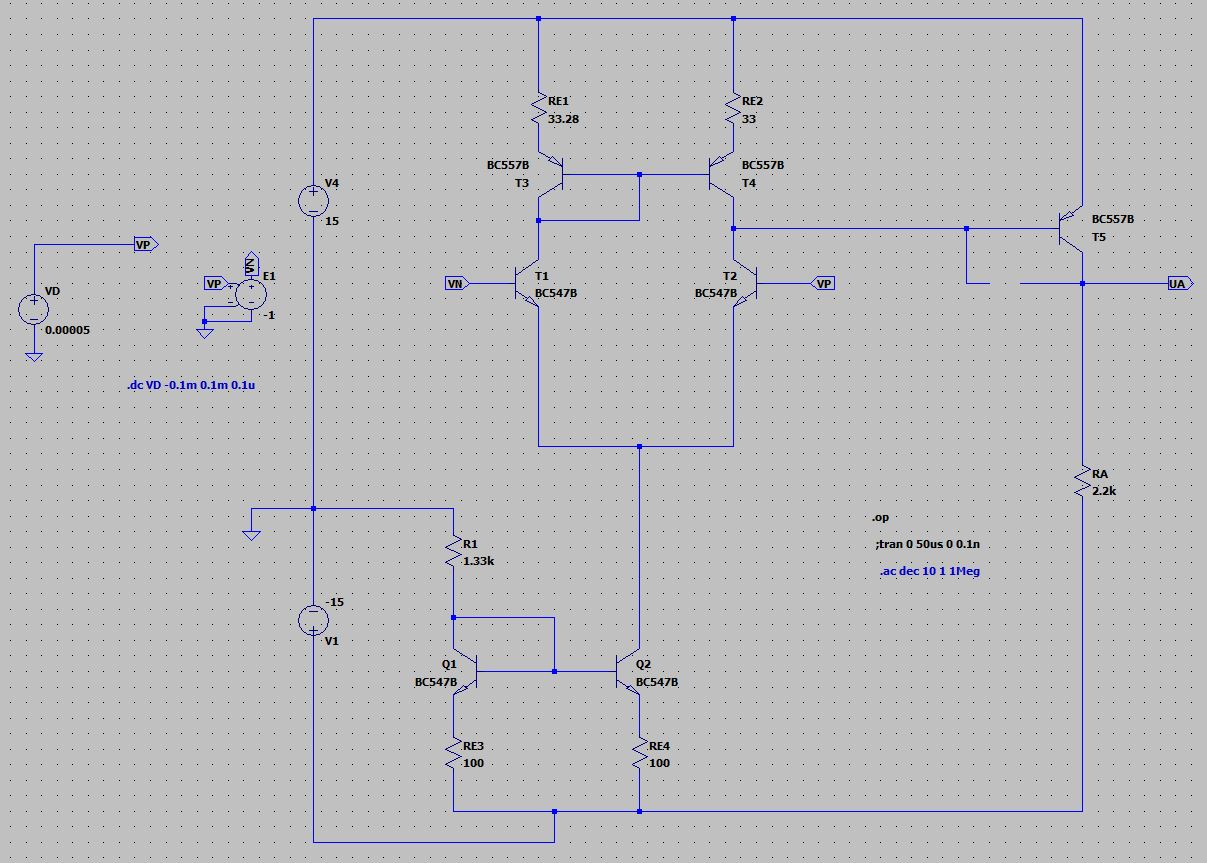
\includegraphics[width = 0.8\textwidth]{\figpath/millerOP.jpg}
    \caption{Schematic des erweiterten OP}
    \label{fig_Kap5_14:SpiceSchematic}
\end{figure}

\begin{figure}[H]
	\centering \small
	\scalebox{0.9}{% This file was created by matlab2tikz.
%
\definecolor{mycolor1}{rgb}{0.00000,0.44700,0.74100}%
%
\begin{tikzpicture}

\begin{axis}[%
width=4.521in,
height=3.566in,
at={(0.758in,0.481in)},
scale only axis,
xmin=-0.2,
xmax=0.05,
xlabel style={font=\color{white!15!black}},
xlabel={$U_d \text{ in } \SI{}{\milli\volt}$},
ymin=-15,
ymax=15,
ylabel style={font=\color{white!15!black}},
ylabel={$U_a \text{ in } \text{V}$},
axis background/.style={fill=white},
title style={font=\bfseries},
title={$U_a$},
xmajorgrids,
ymajorgrids
]
\addplot [color=mycolor1, forget plot]
  table[row sep=crcr]{%
-0.2	-14.99\\
-0.2	-14.99\\
-0.2	-14.99\\
-0.2	-14.99\\
-0.2	-14.99\\
-0.2	-14.99\\
-0.199	-14.99\\
-0.199	-14.99\\
-0.199	-14.99\\
-0.199	-14.99\\
-0.199	-14.99\\
-0.199	-14.99\\
-0.199	-14.99\\
-0.199	-14.99\\
-0.199	-14.99\\
-0.199	-14.99\\
-0.198	-14.99\\
-0.198	-14.99\\
-0.198	-14.99\\
-0.198	-14.99\\
-0.198	-14.99\\
-0.198	-14.99\\
-0.198	-14.99\\
-0.198	-14.99\\
-0.198	-14.99\\
-0.198	-14.99\\
-0.197	-14.99\\
-0.197	-14.99\\
-0.197	-14.99\\
-0.197	-14.99\\
-0.197	-14.99\\
-0.197	-14.99\\
-0.197	-14.99\\
-0.197	-14.99\\
-0.197	-14.99\\
-0.196	-14.98\\
-0.196	-14.98\\
-0.196	-14.98\\
-0.196	-14.98\\
-0.196	-14.98\\
-0.196	-14.98\\
-0.196	-14.98\\
-0.196	-14.98\\
-0.196	-14.98\\
-0.196	-14.98\\
-0.195	-14.98\\
-0.195	-14.98\\
-0.195	-14.98\\
-0.195	-14.98\\
-0.195	-14.98\\
-0.195	-14.98\\
-0.195	-14.98\\
-0.195	-14.98\\
-0.195	-14.98\\
-0.195	-14.98\\
-0.194	-14.98\\
-0.194	-14.98\\
-0.194	-14.98\\
-0.194	-14.98\\
-0.194	-14.98\\
-0.194	-14.98\\
-0.194	-14.98\\
-0.194	-14.98\\
-0.194	-14.98\\
-0.194	-14.98\\
-0.193	-14.98\\
-0.193	-14.98\\
-0.193	-14.98\\
-0.193	-14.98\\
-0.193	-14.98\\
-0.193	-14.98\\
-0.193	-14.98\\
-0.193	-14.98\\
-0.193	-14.97\\
-0.193	-14.97\\
-0.192	-14.97\\
-0.192	-14.97\\
-0.192	-14.97\\
-0.192	-14.97\\
-0.192	-14.97\\
-0.192	-14.97\\
-0.192	-14.97\\
-0.192	-14.97\\
-0.192	-14.97\\
-0.192	-14.97\\
-0.191	-14.97\\
-0.191	-14.97\\
-0.191	-14.97\\
-0.191	-14.97\\
-0.191	-14.97\\
-0.191	-14.97\\
-0.191	-14.97\\
-0.191	-14.97\\
-0.191	-14.97\\
-0.191	-14.97\\
-0.19	-14.97\\
-0.19	-14.97\\
-0.19	-14.97\\
-0.19	-14.97\\
-0.19	-14.96\\
-0.19	-14.96\\
-0.19	-14.96\\
-0.19	-14.96\\
-0.19	-14.96\\
-0.19	-14.96\\
-0.189	-14.96\\
-0.189	-14.96\\
-0.189	-14.96\\
-0.189	-14.96\\
-0.189	-14.96\\
-0.189	-14.96\\
-0.189	-14.96\\
-0.189	-14.96\\
-0.189	-14.96\\
-0.189	-14.96\\
-0.188	-14.96\\
-0.188	-14.96\\
-0.188	-14.96\\
-0.188	-14.95\\
-0.188	-14.95\\
-0.188	-14.95\\
-0.188	-14.95\\
-0.188	-14.95\\
-0.188	-14.95\\
-0.188	-14.95\\
-0.187	-14.95\\
-0.187	-14.95\\
-0.187	-14.95\\
-0.187	-14.95\\
-0.187	-14.95\\
-0.187	-14.95\\
-0.187	-14.95\\
-0.187	-14.95\\
-0.187	-14.94\\
-0.187	-14.94\\
-0.186	-14.94\\
-0.186	-14.94\\
-0.186	-14.94\\
-0.186	-14.94\\
-0.186	-14.94\\
-0.186	-14.94\\
-0.186	-14.94\\
-0.186	-14.94\\
-0.186	-14.94\\
-0.186	-14.94\\
-0.185	-14.93\\
-0.185	-14.93\\
-0.185	-14.93\\
-0.185	-14.93\\
-0.185	-14.93\\
-0.185	-14.93\\
-0.185	-14.93\\
-0.185	-14.93\\
-0.185	-14.93\\
-0.185	-14.93\\
-0.184	-14.93\\
-0.184	-14.92\\
-0.184	-14.92\\
-0.184	-14.92\\
-0.184	-14.92\\
-0.184	-14.92\\
-0.184	-14.92\\
-0.184	-14.92\\
-0.184	-14.92\\
-0.184	-14.92\\
-0.183	-14.92\\
-0.183	-14.91\\
-0.183	-14.91\\
-0.183	-14.91\\
-0.183	-14.91\\
-0.183	-14.91\\
-0.183	-14.91\\
-0.183	-14.91\\
-0.183	-14.91\\
-0.183	-14.9\\
-0.182	-14.9\\
-0.182	-14.9\\
-0.182	-14.9\\
-0.182	-14.9\\
-0.182	-14.9\\
-0.182	-14.9\\
-0.182	-14.9\\
-0.182	-14.89\\
-0.182	-14.89\\
-0.182	-14.89\\
-0.181	-14.89\\
-0.181	-14.89\\
-0.181	-14.89\\
-0.181	-14.89\\
-0.181	-14.88\\
-0.181	-14.88\\
-0.181	-14.88\\
-0.181	-14.88\\
-0.181	-14.88\\
-0.181	-14.88\\
-0.18	-14.87\\
-0.18	-14.87\\
-0.18	-14.87\\
-0.18	-14.87\\
-0.18	-14.87\\
-0.18	-14.87\\
-0.18	-14.86\\
-0.18	-14.86\\
-0.18	-14.86\\
-0.18	-14.86\\
-0.179	-14.86\\
-0.179	-14.85\\
-0.179	-14.85\\
-0.179	-14.85\\
-0.179	-14.85\\
-0.179	-14.85\\
-0.179	-14.85\\
-0.179	-14.84\\
-0.179	-14.84\\
-0.179	-14.84\\
-0.178	-14.84\\
-0.178	-14.83\\
-0.178	-14.83\\
-0.178	-14.83\\
-0.178	-14.83\\
-0.178	-14.83\\
-0.178	-14.82\\
-0.178	-14.82\\
-0.178	-14.82\\
-0.178	-14.82\\
-0.177	-14.81\\
-0.177	-14.81\\
-0.177	-14.81\\
-0.177	-14.81\\
-0.177	-14.8\\
-0.177	-14.8\\
-0.177	-14.8\\
-0.177	-14.8\\
-0.177	-14.79\\
-0.177	-14.79\\
-0.176	-14.79\\
-0.176	-14.79\\
-0.176	-14.78\\
-0.176	-14.78\\
-0.176	-14.78\\
-0.176	-14.78\\
-0.176	-14.77\\
-0.176	-14.77\\
-0.176	-14.77\\
-0.176	-14.76\\
-0.175	-14.76\\
-0.175	-14.76\\
-0.175	-14.75\\
-0.175	-14.75\\
-0.175	-14.75\\
-0.175	-14.74\\
-0.175	-14.74\\
-0.175	-14.74\\
-0.175	-14.74\\
-0.175	-14.73\\
-0.174	-14.73\\
-0.174	-14.72\\
-0.174	-14.72\\
-0.174	-14.72\\
-0.174	-14.71\\
-0.174	-14.71\\
-0.174	-14.71\\
-0.174	-14.7\\
-0.174	-14.7\\
-0.174	-14.7\\
-0.173	-14.69\\
-0.173	-14.69\\
-0.173	-14.68\\
-0.173	-14.68\\
-0.173	-14.68\\
-0.173	-14.67\\
-0.173	-14.67\\
-0.173	-14.66\\
-0.173	-14.66\\
-0.173	-14.66\\
-0.172	-14.65\\
-0.172	-14.65\\
-0.172	-14.64\\
-0.172	-14.64\\
-0.172	-14.63\\
-0.172	-14.63\\
-0.172	-14.62\\
-0.172	-14.62\\
-0.172	-14.62\\
-0.172	-14.61\\
-0.171	-14.61\\
-0.171	-14.6\\
-0.171	-14.6\\
-0.171	-14.59\\
-0.171	-14.59\\
-0.171	-14.58\\
-0.171	-14.58\\
-0.171	-14.57\\
-0.171	-14.57\\
-0.171	-14.56\\
-0.17	-14.55\\
-0.17	-14.55\\
-0.17	-14.54\\
-0.17	-14.54\\
-0.17	-14.53\\
-0.17	-14.53\\
-0.17	-14.52\\
-0.17	-14.52\\
-0.17	-14.51\\
-0.17	-14.5\\
-0.169	-14.5\\
-0.169	-14.49\\
-0.169	-14.49\\
-0.169	-14.48\\
-0.169	-14.47\\
-0.169	-14.47\\
-0.169	-14.46\\
-0.169	-14.45\\
-0.169	-14.45\\
-0.169	-14.44\\
-0.168	-14.44\\
-0.168	-14.43\\
-0.168	-14.42\\
-0.168	-14.41\\
-0.168	-14.41\\
-0.168	-14.4\\
-0.168	-14.39\\
-0.168	-14.39\\
-0.168	-14.38\\
-0.168	-14.37\\
-0.167	-14.37\\
-0.167	-14.36\\
-0.167	-14.35\\
-0.167	-14.34\\
-0.167	-14.34\\
-0.167	-14.33\\
-0.167	-14.32\\
-0.167	-14.31\\
-0.167	-14.3\\
-0.167	-14.3\\
-0.166	-14.29\\
-0.166	-14.28\\
-0.166	-14.27\\
-0.166	-14.26\\
-0.166	-14.26\\
-0.166	-14.25\\
-0.166	-14.24\\
-0.166	-14.23\\
-0.166	-14.22\\
-0.166	-14.21\\
-0.165	-14.2\\
-0.165	-14.2\\
-0.165	-14.19\\
-0.165	-14.18\\
-0.165	-14.17\\
-0.165	-14.16\\
-0.165	-14.15\\
-0.165	-14.14\\
-0.165	-14.13\\
-0.165	-14.12\\
-0.164	-14.11\\
-0.164	-14.1\\
-0.164	-14.09\\
-0.164	-14.08\\
-0.164	-14.07\\
-0.164	-14.06\\
-0.164	-14.05\\
-0.164	-14.04\\
-0.164	-14.03\\
-0.164	-14.02\\
-0.163	-14.01\\
-0.163	-14\\
-0.163	-13.99\\
-0.163	-13.98\\
-0.163	-13.97\\
-0.163	-13.96\\
-0.163	-13.95\\
-0.163	-13.93\\
-0.163	-13.92\\
-0.163	-13.91\\
-0.162	-13.9\\
-0.162	-13.89\\
-0.162	-13.88\\
-0.162	-13.87\\
-0.162	-13.85\\
-0.162	-13.84\\
-0.162	-13.83\\
-0.162	-13.82\\
-0.162	-13.81\\
-0.162	-13.79\\
-0.161	-13.78\\
-0.161	-13.77\\
-0.161	-13.76\\
-0.161	-13.74\\
-0.161	-13.73\\
-0.161	-13.72\\
-0.161	-13.71\\
-0.161	-13.69\\
-0.161	-13.68\\
-0.161	-13.67\\
-0.16	-13.65\\
-0.16	-13.64\\
-0.16	-13.63\\
-0.16	-13.61\\
-0.16	-13.6\\
-0.16	-13.59\\
-0.16	-13.57\\
-0.16	-13.56\\
-0.16	-13.54\\
-0.16	-13.53\\
-0.159	-13.52\\
-0.159	-13.5\\
-0.159	-13.49\\
-0.159	-13.47\\
-0.159	-13.46\\
-0.159	-13.44\\
-0.159	-13.43\\
-0.159	-13.41\\
-0.159	-13.4\\
-0.159	-13.39\\
-0.158	-13.37\\
-0.158	-13.35\\
-0.158	-13.34\\
-0.158	-13.32\\
-0.158	-13.31\\
-0.158	-13.29\\
-0.158	-13.28\\
-0.158	-13.26\\
-0.158	-13.25\\
-0.158	-13.23\\
-0.157	-13.21\\
-0.157	-13.2\\
-0.157	-13.18\\
-0.157	-13.17\\
-0.157	-13.15\\
-0.157	-13.13\\
-0.157	-13.12\\
-0.157	-13.1\\
-0.157	-13.08\\
-0.157	-13.07\\
-0.156	-13.05\\
-0.156	-13.03\\
-0.156	-13.01\\
-0.156	-13\\
-0.156	-12.98\\
-0.156	-12.96\\
-0.156	-12.94\\
-0.156	-12.93\\
-0.156	-12.91\\
-0.156	-12.89\\
-0.155	-12.87\\
-0.155	-12.86\\
-0.155	-12.84\\
-0.155	-12.82\\
-0.155	-12.8\\
-0.155	-12.78\\
-0.155	-12.77\\
-0.155	-12.75\\
-0.155	-12.73\\
-0.155	-12.71\\
-0.154	-12.69\\
-0.154	-12.67\\
-0.154	-12.65\\
-0.154	-12.63\\
-0.154	-12.61\\
-0.154	-12.6\\
-0.154	-12.58\\
-0.154	-12.56\\
-0.154	-12.54\\
-0.154	-12.52\\
-0.153	-12.5\\
-0.153	-12.48\\
-0.153	-12.46\\
-0.153	-12.44\\
-0.153	-12.42\\
-0.153	-12.4\\
-0.153	-12.38\\
-0.153	-12.36\\
-0.153	-12.34\\
-0.153	-12.32\\
-0.152	-12.3\\
-0.152	-12.28\\
-0.152	-12.26\\
-0.152	-12.24\\
-0.152	-12.22\\
-0.152	-12.2\\
-0.152	-12.17\\
-0.152	-12.15\\
-0.152	-12.13\\
-0.152	-12.11\\
-0.151	-12.09\\
-0.151	-12.07\\
-0.151	-12.05\\
-0.151	-12.03\\
-0.151	-12.01\\
-0.151	-11.98\\
-0.151	-11.96\\
-0.151	-11.94\\
-0.151	-11.92\\
-0.151	-11.9\\
-0.15	-11.87\\
-0.15	-11.85\\
-0.15	-11.83\\
-0.15	-11.81\\
-0.15	-11.79\\
-0.15	-11.76\\
-0.15	-11.74\\
-0.15	-11.72\\
-0.15	-11.7\\
-0.15	-11.67\\
-0.149	-11.65\\
-0.149	-11.63\\
-0.149	-11.61\\
-0.149	-11.58\\
-0.149	-11.56\\
-0.149	-11.54\\
-0.149	-11.52\\
-0.149	-11.49\\
-0.149	-11.47\\
-0.149	-11.45\\
-0.148	-11.42\\
-0.148	-11.4\\
-0.148	-11.38\\
-0.148	-11.35\\
-0.148	-11.33\\
-0.148	-11.31\\
-0.148	-11.28\\
-0.148	-11.26\\
-0.148	-11.24\\
-0.148	-11.21\\
-0.147	-11.19\\
-0.147	-11.16\\
-0.147	-11.14\\
-0.147	-11.12\\
-0.147	-11.09\\
-0.147	-11.07\\
-0.147	-11.04\\
-0.147	-11.02\\
-0.147	-11\\
-0.147	-10.97\\
-0.146	-10.95\\
-0.146	-10.92\\
-0.146	-10.9\\
-0.146	-10.87\\
-0.146	-10.85\\
-0.146	-10.83\\
-0.146	-10.8\\
-0.146	-10.78\\
-0.146	-10.75\\
-0.146	-10.73\\
-0.145	-10.7\\
-0.145	-10.68\\
-0.145	-10.65\\
-0.145	-10.63\\
-0.145	-10.6\\
-0.145	-10.58\\
-0.145	-10.55\\
-0.145	-10.53\\
-0.145	-10.5\\
-0.145	-10.48\\
-0.144	-10.45\\
-0.144	-10.43\\
-0.144	-10.4\\
-0.144	-10.38\\
-0.144	-10.35\\
-0.144	-10.33\\
-0.144	-10.3\\
-0.144	-10.27\\
-0.144	-10.25\\
-0.144	-10.22\\
-0.143	-10.2\\
-0.143	-10.17\\
-0.143	-10.15\\
-0.143	-10.12\\
-0.143	-10.1\\
-0.143	-10.07\\
-0.143	-10.04\\
-0.143	-10.02\\
-0.143	-9.99\\
-0.143	-9.97\\
-0.142	-9.94\\
-0.142	-9.91\\
-0.142	-9.89\\
-0.142	-9.86\\
-0.142	-9.84\\
-0.142	-9.81\\
-0.142	-9.78\\
-0.142	-9.76\\
-0.142	-9.73\\
-0.142	-9.71\\
-0.141	-9.68\\
-0.141	-9.65\\
-0.141	-9.63\\
-0.141	-9.6\\
-0.141	-9.57\\
-0.141	-9.55\\
-0.141	-9.52\\
-0.141	-9.5\\
-0.141	-9.47\\
-0.141	-9.44\\
-0.14	-9.42\\
-0.14	-9.39\\
-0.14	-9.36\\
-0.14	-9.34\\
-0.14	-9.31\\
-0.14	-9.28\\
-0.14	-9.26\\
-0.14	-9.23\\
-0.14	-9.2\\
-0.14	-9.18\\
-0.139	-9.15\\
-0.139	-9.12\\
-0.139	-9.1\\
-0.139	-9.07\\
-0.139	-9.04\\
-0.139	-9.02\\
-0.139	-8.99\\
-0.139	-8.96\\
-0.139	-8.94\\
-0.139	-8.91\\
-0.138	-8.88\\
-0.138	-8.86\\
-0.138	-8.83\\
-0.138	-8.8\\
-0.138	-8.78\\
-0.138	-8.75\\
-0.138	-8.72\\
-0.138	-8.69\\
-0.138	-8.67\\
-0.138	-8.64\\
-0.137	-8.61\\
-0.137	-8.59\\
-0.137	-8.56\\
-0.137	-8.53\\
-0.137	-8.51\\
-0.137	-8.48\\
-0.137	-8.45\\
-0.137	-8.42\\
-0.137	-8.4\\
-0.137	-8.37\\
-0.136	-8.34\\
-0.136	-8.32\\
-0.136	-8.29\\
-0.136	-8.26\\
-0.136	-8.23\\
-0.136	-8.21\\
-0.136	-8.18\\
-0.136	-8.15\\
-0.136	-8.13\\
-0.136	-8.1\\
-0.135	-8.07\\
-0.135	-8.04\\
-0.135	-8.02\\
-0.135	-7.99\\
-0.135	-7.96\\
-0.135	-7.94\\
-0.135	-7.91\\
-0.135	-7.88\\
-0.135	-7.85\\
-0.135	-7.83\\
-0.134	-7.8\\
-0.134	-7.77\\
-0.134	-7.75\\
-0.134	-7.72\\
-0.134	-7.69\\
-0.134	-7.66\\
-0.134	-7.64\\
-0.134	-7.61\\
-0.134	-7.58\\
-0.134	-7.56\\
-0.133	-7.53\\
-0.133	-7.5\\
-0.133	-7.47\\
-0.133	-7.45\\
-0.133	-7.42\\
-0.133	-7.39\\
-0.133	-7.36\\
-0.133	-7.34\\
-0.133	-7.31\\
-0.133	-7.28\\
-0.132	-7.26\\
-0.132	-7.23\\
-0.132	-7.2\\
-0.132	-7.17\\
-0.132	-7.15\\
-0.132	-7.12\\
-0.132	-7.09\\
-0.132	-7.07\\
-0.132	-7.04\\
-0.132	-7.01\\
-0.131	-6.98\\
-0.131	-6.96\\
-0.131	-6.93\\
-0.131	-6.9\\
-0.131	-6.88\\
-0.131	-6.85\\
-0.131	-6.82\\
-0.131	-6.79\\
-0.131	-6.77\\
-0.131	-6.74\\
-0.13	-6.71\\
-0.13	-6.69\\
-0.13	-6.66\\
-0.13	-6.63\\
-0.13	-6.6\\
-0.13	-6.58\\
-0.13	-6.55\\
-0.13	-6.52\\
-0.13	-6.5\\
-0.13	-6.47\\
-0.129	-6.44\\
-0.129	-6.41\\
-0.129	-6.39\\
-0.129	-6.36\\
-0.129	-6.33\\
-0.129	-6.31\\
-0.129	-6.28\\
-0.129	-6.25\\
-0.129	-6.23\\
-0.129	-6.2\\
-0.128	-6.17\\
-0.128	-6.14\\
-0.128	-6.12\\
-0.128	-6.09\\
-0.128	-6.06\\
-0.128	-6.04\\
-0.128	-6.01\\
-0.128	-5.98\\
-0.128	-5.96\\
-0.128	-5.93\\
-0.127	-5.9\\
-0.127	-5.88\\
-0.127	-5.85\\
-0.127	-5.82\\
-0.127	-5.8\\
-0.127	-5.77\\
-0.127	-5.74\\
-0.127	-5.72\\
-0.127	-5.69\\
-0.127	-5.66\\
-0.126	-5.64\\
-0.126	-5.61\\
-0.126	-5.58\\
-0.126	-5.56\\
-0.126	-5.53\\
-0.126	-5.5\\
-0.126	-5.48\\
-0.126	-5.45\\
-0.126	-5.42\\
-0.126	-5.4\\
-0.125	-5.37\\
-0.125	-5.34\\
-0.125	-5.32\\
-0.125	-5.29\\
-0.125	-5.26\\
-0.125	-5.24\\
-0.125	-5.21\\
-0.125	-5.18\\
-0.125	-5.16\\
-0.125	-5.13\\
-0.124	-5.1\\
-0.124	-5.08\\
-0.124	-5.05\\
-0.124	-5.02\\
-0.124	-5\\
-0.124	-4.97\\
-0.124	-4.95\\
-0.124	-4.92\\
-0.124	-4.89\\
-0.124	-4.87\\
-0.123	-4.84\\
-0.123	-4.81\\
-0.123	-4.79\\
-0.123	-4.76\\
-0.123	-4.74\\
-0.123	-4.71\\
-0.123	-4.68\\
-0.123	-4.66\\
-0.123	-4.63\\
-0.123	-4.61\\
-0.122	-4.58\\
-0.122	-4.55\\
-0.122	-4.53\\
-0.122	-4.5\\
-0.122	-4.47\\
-0.122	-4.45\\
-0.122	-4.42\\
-0.122	-4.4\\
-0.122	-4.37\\
-0.122	-4.35\\
-0.121	-4.32\\
-0.121	-4.29\\
-0.121	-4.27\\
-0.121	-4.24\\
-0.121	-4.22\\
-0.121	-4.19\\
-0.121	-4.16\\
-0.121	-4.14\\
-0.121	-4.11\\
-0.121	-4.09\\
-0.12	-4.06\\
-0.12	-4.04\\
-0.12	-4.01\\
-0.12	-3.98\\
-0.12	-3.96\\
-0.12	-3.93\\
-0.12	-3.91\\
-0.12	-3.88\\
-0.12	-3.86\\
-0.12	-3.83\\
-0.119	-3.81\\
-0.119	-3.78\\
-0.119	-3.75\\
-0.119	-3.73\\
-0.119	-3.7\\
-0.119	-3.68\\
-0.119	-3.65\\
-0.119	-3.63\\
-0.119	-3.6\\
-0.119	-3.58\\
-0.118	-3.55\\
-0.118	-3.53\\
-0.118	-3.5\\
-0.118	-3.48\\
-0.118	-3.45\\
-0.118	-3.42\\
-0.118	-3.4\\
-0.118	-3.37\\
-0.118	-3.35\\
-0.118	-3.32\\
-0.117	-3.3\\
-0.117	-3.27\\
-0.117	-3.25\\
-0.117	-3.22\\
-0.117	-3.2\\
-0.117	-3.17\\
-0.117	-3.15\\
-0.117	-3.12\\
-0.117	-3.1\\
-0.117	-3.07\\
-0.116	-3.05\\
-0.116	-3.02\\
-0.116	-3\\
-0.116	-2.97\\
-0.116	-2.95\\
-0.116	-2.93\\
-0.116	-2.9\\
-0.116	-2.88\\
-0.116	-2.85\\
-0.116	-2.83\\
-0.115	-2.8\\
-0.115	-2.78\\
-0.115	-2.75\\
-0.115	-2.73\\
-0.115	-2.7\\
-0.115	-2.68\\
-0.115	-2.65\\
-0.115	-2.63\\
-0.115	-2.6\\
-0.115	-2.58\\
-0.114	-2.56\\
-0.114	-2.53\\
-0.114	-2.51\\
-0.114	-2.48\\
-0.114	-2.46\\
-0.114	-2.43\\
-0.114	-2.41\\
-0.114	-2.39\\
-0.114	-2.36\\
-0.114	-2.34\\
-0.113	-2.31\\
-0.113	-2.29\\
-0.113	-2.26\\
-0.113	-2.24\\
-0.113	-2.22\\
-0.113	-2.19\\
-0.113	-2.17\\
-0.113	-2.14\\
-0.113	-2.12\\
-0.113	-2.1\\
-0.112	-2.07\\
-0.112	-2.05\\
-0.112	-2.02\\
-0.112	-2\\
-0.112	-1.98\\
-0.112	-1.95\\
-0.112	-1.93\\
-0.112	-1.9\\
-0.112	-1.88\\
-0.112	-1.86\\
-0.111	-1.83\\
-0.111	-1.81\\
-0.111	-1.79\\
-0.111	-1.76\\
-0.111	-1.74\\
-0.111	-1.71\\
-0.111	-1.69\\
-0.111	-1.67\\
-0.111	-1.64\\
-0.111	-1.62\\
-0.11	-1.6\\
-0.11	-1.57\\
-0.11	-1.55\\
-0.11	-1.53\\
-0.11	-1.5\\
-0.11	-1.48\\
-0.11	-1.46\\
-0.11	-1.43\\
-0.11	-1.41\\
-0.11	-1.39\\
-0.109	-1.36\\
-0.109	-1.34\\
-0.109	-1.32\\
-0.109	-1.29\\
-0.109	-1.27\\
-0.109	-1.25\\
-0.109	-1.22\\
-0.109	-1.2\\
-0.109	-1.18\\
-0.109	-1.15\\
-0.108	-1.13\\
-0.108	-1.11\\
-0.108	-1.08\\
-0.108	-1.06\\
-0.108	-1.04\\
-0.108	-1.02\\
-0.108	-0.99\\
-0.108	-0.97\\
-0.108	-0.95\\
-0.108	-0.92\\
-0.107	-0.9\\
-0.107	-0.88\\
-0.107	-0.86\\
-0.107	-0.83\\
-0.107	-0.81\\
-0.107	-0.79\\
-0.107	-0.76\\
-0.107	-0.74\\
-0.107	-0.72\\
-0.107	-0.7\\
-0.106	-0.67\\
-0.106	-0.65\\
-0.106	-0.63\\
-0.106	-0.61\\
-0.106	-0.58\\
-0.106	-0.56\\
-0.106	-0.54\\
-0.106	-0.52\\
-0.106	-0.49\\
-0.106	-0.47\\
-0.105	-0.45\\
-0.105	-0.43\\
-0.105	-0.4\\
-0.105	-0.38\\
-0.105	-0.36\\
-0.105	-0.34\\
-0.105	-0.32\\
-0.105	-0.29\\
-0.105	-0.27\\
-0.105	-0.25\\
-0.104	-0.23\\
-0.104	-0.2\\
-0.104	-0.18\\
-0.104	-0.16\\
-0.104	-0.14\\
-0.104	-0.12\\
-0.104	-0.09\\
-0.104	-0.07\\
-0.104	-0.05\\
-0.104	-0.03\\
-0.103	-0.01\\
-0.103	0.01\\
-0.103	0.04\\
-0.103	0.06\\
-0.103	0.08\\
-0.103	0.1\\
-0.103	0.12\\
-0.103	0.15\\
-0.103	0.17\\
-0.103	0.19\\
-0.102	0.21\\
-0.102	0.23\\
-0.102	0.25\\
-0.102	0.28\\
-0.102	0.3\\
-0.102	0.32\\
-0.102	0.34\\
-0.102	0.36\\
-0.102	0.38\\
-0.102	0.4\\
-0.101	0.43\\
-0.101	0.45\\
-0.101	0.47\\
-0.101	0.49\\
-0.101	0.51\\
-0.101	0.53\\
-0.101	0.55\\
-0.101	0.58\\
-0.101	0.6\\
-0.101	0.62\\
-0.1	0.64\\
-0.1	0.66\\
-0.1	0.68\\
-0.1	0.7\\
-0.1	0.72\\
-0.1	0.75\\
-0.1	0.77\\
-0.1	0.79\\
-0.1	0.81\\
-0.1	0.83\\
-0.099	0.85\\
-0.099	0.87\\
-0.099	0.89\\
-0.099	0.91\\
-0.099	0.93\\
-0.099	0.95\\
-0.099	0.98\\
-0.099	1\\
-0.099	1.02\\
-0.099	1.04\\
-0.098	1.06\\
-0.098	1.08\\
-0.098	1.1\\
-0.098	1.12\\
-0.098	1.14\\
-0.098	1.16\\
-0.098	1.18\\
-0.098	1.2\\
-0.098	1.22\\
-0.098	1.24\\
-0.097	1.27\\
-0.097	1.29\\
-0.097	1.31\\
-0.097	1.33\\
-0.097	1.35\\
-0.097	1.37\\
-0.097	1.39\\
-0.097	1.41\\
-0.097	1.43\\
-0.097	1.45\\
-0.096	1.47\\
-0.096	1.49\\
-0.096	1.51\\
-0.096	1.53\\
-0.096	1.55\\
-0.096	1.57\\
-0.096	1.59\\
-0.096	1.61\\
-0.096	1.63\\
-0.096	1.65\\
-0.095	1.67\\
-0.095	1.69\\
-0.095	1.71\\
-0.095	1.73\\
-0.095	1.75\\
-0.095	1.77\\
-0.095	1.79\\
-0.095	1.81\\
-0.095	1.83\\
-0.095	1.85\\
-0.094	1.87\\
-0.094	1.89\\
-0.094	1.91\\
-0.094	1.93\\
-0.094	1.95\\
-0.094	1.97\\
-0.094	1.99\\
-0.094	2.01\\
-0.094	2.03\\
-0.094	2.05\\
-0.093	2.07\\
-0.093	2.09\\
-0.093	2.11\\
-0.093	2.13\\
-0.093	2.15\\
-0.093	2.17\\
-0.093	2.19\\
-0.093	2.2\\
-0.093	2.22\\
-0.093	2.24\\
-0.092	2.26\\
-0.092	2.28\\
-0.092	2.3\\
-0.092	2.32\\
-0.092	2.34\\
-0.092	2.36\\
-0.092	2.38\\
-0.092	2.4\\
-0.092	2.42\\
-0.092	2.44\\
-0.091	2.46\\
-0.091	2.48\\
-0.091	2.49\\
-0.091	2.51\\
-0.091	2.53\\
-0.091	2.55\\
-0.091	2.57\\
-0.091	2.59\\
-0.091	2.61\\
-0.091	2.63\\
-0.09	2.65\\
-0.09	2.67\\
-0.09	2.69\\
-0.09	2.7\\
-0.09	2.72\\
-0.09	2.74\\
-0.09	2.76\\
-0.09	2.78\\
-0.09	2.8\\
-0.09	2.82\\
-0.089	2.84\\
-0.089	2.85\\
-0.089	2.87\\
-0.089	2.89\\
-0.089	2.91\\
-0.089	2.93\\
-0.089	2.95\\
-0.089	2.97\\
-0.089	2.99\\
-0.089	3\\
-0.088	3.02\\
-0.088	3.04\\
-0.088	3.06\\
-0.088	3.08\\
-0.088	3.1\\
-0.088	3.12\\
-0.088	3.13\\
-0.088	3.15\\
-0.088	3.17\\
-0.088	3.19\\
-0.087	3.21\\
-0.087	3.23\\
-0.087	3.24\\
-0.087	3.26\\
-0.087	3.28\\
-0.087	3.3\\
-0.087	3.32\\
-0.087	3.34\\
-0.087	3.35\\
-0.087	3.37\\
-0.086	3.39\\
-0.086	3.41\\
-0.086	3.43\\
-0.086	3.44\\
-0.086	3.46\\
-0.086	3.48\\
-0.086	3.5\\
-0.086	3.52\\
-0.086	3.53\\
-0.086	3.55\\
-0.085	3.57\\
-0.085	3.59\\
-0.085	3.61\\
-0.085	3.62\\
-0.085	3.64\\
-0.085	3.66\\
-0.085	3.68\\
-0.085	3.7\\
-0.085	3.71\\
-0.085	3.73\\
-0.084	3.75\\
-0.084	3.77\\
-0.084	3.78\\
-0.084	3.8\\
-0.084	3.82\\
-0.084	3.84\\
-0.084	3.86\\
-0.084	3.87\\
-0.084	3.89\\
-0.084	3.91\\
-0.083	3.93\\
-0.083	3.94\\
-0.083	3.96\\
-0.083	3.98\\
-0.083	4\\
-0.083	4.01\\
-0.083	4.03\\
-0.083	4.05\\
-0.083	4.07\\
-0.083	4.08\\
-0.082	4.1\\
-0.082	4.12\\
-0.082	4.13\\
-0.082	4.15\\
-0.082	4.17\\
-0.082	4.19\\
-0.082	4.2\\
-0.082	4.22\\
-0.082	4.24\\
-0.082	4.26\\
-0.081	4.27\\
-0.081	4.29\\
-0.081	4.31\\
-0.081	4.32\\
-0.081	4.34\\
-0.081	4.36\\
-0.081	4.38\\
-0.081	4.39\\
-0.081	4.41\\
-0.081	4.43\\
-0.08	4.44\\
-0.08	4.46\\
-0.08	4.48\\
-0.08	4.49\\
-0.08	4.51\\
-0.08	4.53\\
-0.08	4.55\\
-0.08	4.56\\
-0.08	4.58\\
-0.08	4.6\\
-0.079	4.61\\
-0.079	4.63\\
-0.079	4.65\\
-0.079	4.66\\
-0.079	4.68\\
-0.079	4.7\\
-0.079	4.71\\
-0.079	4.73\\
-0.079	4.75\\
-0.079	4.76\\
-0.078	4.78\\
-0.078	4.8\\
-0.078	4.81\\
-0.078	4.83\\
-0.078	4.85\\
-0.078	4.86\\
-0.078	4.88\\
-0.078	4.9\\
-0.078	4.91\\
-0.078	4.93\\
-0.077	4.94\\
-0.077	4.96\\
-0.077	4.98\\
-0.077	4.99\\
-0.077	5.01\\
-0.077	5.03\\
-0.077	5.04\\
-0.077	5.06\\
-0.077	5.08\\
-0.077	5.09\\
-0.076	5.11\\
-0.076	5.12\\
-0.076	5.14\\
-0.076	5.16\\
-0.076	5.17\\
-0.076	5.19\\
-0.076	5.21\\
-0.076	5.22\\
-0.076	5.24\\
-0.076	5.25\\
-0.075	5.27\\
-0.075	5.29\\
-0.075	5.3\\
-0.075	5.32\\
-0.075	5.33\\
-0.075	5.35\\
-0.075	5.37\\
-0.075	5.38\\
-0.075	5.4\\
-0.075	5.41\\
-0.074	5.43\\
-0.074	5.45\\
-0.074	5.46\\
-0.074	5.48\\
-0.074	5.49\\
-0.074	5.51\\
-0.074	5.52\\
-0.074	5.54\\
-0.074	5.56\\
-0.074	5.57\\
-0.073	5.59\\
-0.073	5.6\\
-0.073	5.62\\
-0.073	5.63\\
-0.073	5.65\\
-0.073	5.67\\
-0.073	5.68\\
-0.073	5.7\\
-0.073	5.71\\
-0.073	5.73\\
-0.072	5.74\\
-0.072	5.76\\
-0.072	5.78\\
-0.072	5.79\\
-0.072	5.81\\
-0.072	5.82\\
-0.072	5.84\\
-0.072	5.85\\
-0.072	5.87\\
-0.072	5.88\\
-0.071	5.9\\
-0.071	5.91\\
-0.071	5.93\\
-0.071	5.94\\
-0.071	5.96\\
-0.071	5.98\\
-0.071	5.99\\
-0.071	6.01\\
-0.071	6.02\\
-0.071	6.04\\
-0.07	6.05\\
-0.07	6.07\\
-0.07	6.08\\
-0.07	6.1\\
-0.07	6.11\\
-0.07	6.13\\
-0.07	6.14\\
-0.07	6.16\\
-0.07	6.17\\
-0.07	6.19\\
-0.069	6.2\\
-0.069	6.22\\
-0.069	6.23\\
-0.069	6.25\\
-0.069	6.26\\
-0.069	6.28\\
-0.069	6.29\\
-0.069	6.31\\
-0.069	6.32\\
-0.069	6.34\\
-0.068	6.35\\
-0.068	6.37\\
-0.068	6.38\\
-0.068	6.4\\
-0.068	6.41\\
-0.068	6.43\\
-0.068	6.44\\
-0.068	6.46\\
-0.068	6.47\\
-0.068	6.49\\
-0.067	6.5\\
-0.067	6.52\\
-0.067	6.53\\
-0.067	6.55\\
-0.067	6.56\\
-0.067	6.57\\
-0.067	6.59\\
-0.067	6.6\\
-0.067	6.62\\
-0.067	6.63\\
-0.066	6.65\\
-0.066	6.66\\
-0.066	6.68\\
-0.066	6.69\\
-0.066	6.71\\
-0.066	6.72\\
-0.066	6.73\\
-0.066	6.75\\
-0.066	6.76\\
-0.066	6.78\\
-0.065	6.79\\
-0.065	6.81\\
-0.065	6.82\\
-0.065	6.84\\
-0.065	6.85\\
-0.065	6.86\\
-0.065	6.88\\
-0.065	6.89\\
-0.065	6.91\\
-0.065	6.92\\
-0.064	6.94\\
-0.064	6.95\\
-0.064	6.96\\
-0.064	6.98\\
-0.064	6.99\\
-0.064	7.01\\
-0.064	7.02\\
-0.064	7.04\\
-0.064	7.05\\
-0.064	7.06\\
-0.063	7.08\\
-0.063	7.09\\
-0.063	7.11\\
-0.063	7.12\\
-0.063	7.13\\
-0.063	7.15\\
-0.063	7.16\\
-0.063	7.18\\
-0.063	7.19\\
-0.063	7.2\\
-0.062	7.22\\
-0.062	7.23\\
-0.062	7.25\\
-0.062	7.26\\
-0.062	7.27\\
-0.062	7.29\\
-0.062	7.3\\
-0.062	7.32\\
-0.062	7.33\\
-0.062	7.34\\
-0.061	7.36\\
-0.061	7.37\\
-0.061	7.38\\
-0.061	7.4\\
-0.061	7.41\\
-0.061	7.43\\
-0.061	7.44\\
-0.061	7.45\\
-0.061	7.47\\
-0.061	7.48\\
-0.06	7.49\\
-0.06	7.51\\
-0.06	7.52\\
-0.06	7.54\\
-0.06	7.55\\
-0.06	7.56\\
-0.06	7.58\\
-0.06	7.59\\
-0.06	7.6\\
-0.06	7.62\\
-0.059	7.63\\
-0.059	7.64\\
-0.059	7.66\\
-0.059	7.67\\
-0.059	7.68\\
-0.059	7.7\\
-0.059	7.71\\
-0.059	7.72\\
-0.059	7.74\\
-0.059	7.75\\
-0.058	7.76\\
-0.058	7.78\\
-0.058	7.79\\
-0.058	7.8\\
-0.058	7.82\\
-0.058	7.83\\
-0.058	7.84\\
-0.058	7.86\\
-0.058	7.87\\
-0.058	7.88\\
-0.057	7.9\\
-0.057	7.91\\
-0.057	7.92\\
-0.057	7.94\\
-0.057	7.95\\
-0.057	7.96\\
-0.057	7.98\\
-0.057	7.99\\
-0.057	8\\
-0.057	8.02\\
-0.056	8.03\\
-0.056	8.04\\
-0.056	8.06\\
-0.056	8.07\\
-0.056	8.08\\
-0.056	8.09\\
-0.056	8.11\\
-0.056	8.12\\
-0.056	8.13\\
-0.056	8.15\\
-0.055	8.16\\
-0.055	8.17\\
-0.055	8.19\\
-0.055	8.2\\
-0.055	8.21\\
-0.055	8.22\\
-0.055	8.24\\
-0.055	8.25\\
-0.055	8.26\\
-0.055	8.28\\
-0.054	8.29\\
-0.054	8.3\\
-0.054	8.31\\
-0.054	8.33\\
-0.054	8.34\\
-0.054	8.35\\
-0.054	8.37\\
-0.054	8.38\\
-0.054	8.39\\
-0.054	8.4\\
-0.053	8.42\\
-0.053	8.43\\
-0.053	8.44\\
-0.053	8.45\\
-0.053	8.47\\
-0.053	8.48\\
-0.053	8.49\\
-0.053	8.51\\
-0.053	8.52\\
-0.053	8.53\\
-0.052	8.54\\
-0.052	8.56\\
-0.052	8.57\\
-0.052	8.58\\
-0.052	8.59\\
-0.052	8.61\\
-0.052	8.62\\
-0.052	8.63\\
-0.052	8.64\\
-0.052	8.66\\
-0.051	8.67\\
-0.051	8.68\\
-0.051	8.69\\
-0.051	8.71\\
-0.051	8.72\\
-0.051	8.73\\
-0.051	8.74\\
-0.051	8.75\\
-0.051	8.77\\
-0.051	8.78\\
-0.05	8.79\\
-0.05	8.8\\
-0.05	8.82\\
-0.05	8.83\\
-0.05	8.84\\
-0.05	8.85\\
-0.05	8.87\\
-0.05	8.88\\
-0.05	8.89\\
-0.05	8.9\\
-0.049	8.91\\
-0.049	8.93\\
-0.049	8.94\\
-0.049	8.95\\
-0.049	8.96\\
-0.049	8.98\\
-0.049	8.99\\
-0.049	9\\
-0.049	9.01\\
-0.049	9.02\\
-0.048	9.04\\
-0.048	9.05\\
-0.048	9.06\\
-0.048	9.07\\
-0.048	9.08\\
-0.048	9.1\\
-0.048	9.11\\
-0.048	9.12\\
-0.048	9.13\\
-0.048	9.14\\
-0.047	9.16\\
-0.047	9.17\\
-0.047	9.18\\
-0.047	9.19\\
-0.047	9.2\\
-0.047	9.22\\
-0.047	9.23\\
-0.047	9.24\\
-0.047	9.25\\
-0.047	9.26\\
-0.046	9.27\\
-0.046	9.29\\
-0.046	9.3\\
-0.046	9.31\\
-0.046	9.32\\
-0.046	9.33\\
-0.046	9.35\\
-0.046	9.36\\
-0.046	9.37\\
-0.046	9.38\\
-0.045	9.39\\
-0.045	9.4\\
-0.045	9.42\\
-0.045	9.43\\
-0.045	9.44\\
-0.045	9.45\\
-0.045	9.46\\
-0.045	9.47\\
-0.045	9.49\\
-0.045	9.5\\
-0.044	9.51\\
-0.044	9.52\\
-0.044	9.53\\
-0.044	9.54\\
-0.044	9.56\\
-0.044	9.57\\
-0.044	9.58\\
-0.044	9.59\\
-0.044	9.6\\
-0.044	9.61\\
-0.043	9.62\\
-0.043	9.64\\
-0.043	9.65\\
-0.043	9.66\\
-0.043	9.67\\
-0.043	9.68\\
-0.043	9.69\\
-0.043	9.7\\
-0.043	9.72\\
-0.043	9.73\\
-0.042	9.74\\
-0.042	9.75\\
-0.042	9.76\\
-0.042	9.77\\
-0.042	9.78\\
-0.042	9.8\\
-0.042	9.81\\
-0.042	9.82\\
-0.042	9.83\\
-0.042	9.84\\
-0.041	9.85\\
-0.041	9.86\\
-0.041	9.87\\
-0.041	9.89\\
-0.041	9.9\\
-0.041	9.91\\
-0.041	9.92\\
-0.041	9.93\\
-0.041	9.94\\
-0.041	9.95\\
-0.04	9.96\\
-0.04	9.97\\
-0.04	9.99\\
-0.04	10\\
-0.04	10.01\\
-0.04	10.02\\
-0.04	10.03\\
-0.04	10.04\\
-0.04	10.05\\
-0.04	10.06\\
-0.039	10.07\\
-0.039	10.09\\
-0.039	10.1\\
-0.039	10.11\\
-0.039	10.12\\
-0.039	10.13\\
-0.039	10.14\\
-0.039	10.15\\
-0.039	10.16\\
-0.039	10.17\\
-0.038	10.18\\
-0.038	10.2\\
-0.038	10.21\\
-0.038	10.22\\
-0.038	10.23\\
-0.038	10.24\\
-0.038	10.25\\
-0.038	10.26\\
-0.038	10.27\\
-0.038	10.28\\
-0.037	10.29\\
-0.037	10.3\\
-0.037	10.31\\
-0.037	10.33\\
-0.037	10.34\\
-0.037	10.35\\
-0.037	10.36\\
-0.037	10.37\\
-0.037	10.38\\
-0.037	10.39\\
-0.036	10.4\\
-0.036	10.41\\
-0.036	10.42\\
-0.036	10.43\\
-0.036	10.44\\
-0.036	10.45\\
-0.036	10.46\\
-0.036	10.48\\
-0.036	10.49\\
-0.036	10.5\\
-0.035	10.51\\
-0.035	10.52\\
-0.035	10.53\\
-0.035	10.54\\
-0.035	10.55\\
-0.035	10.56\\
-0.035	10.57\\
-0.035	10.58\\
-0.035	10.59\\
-0.035	10.6\\
-0.034	10.61\\
-0.034	10.62\\
-0.034	10.63\\
-0.034	10.64\\
-0.034	10.66\\
-0.034	10.67\\
-0.034	10.68\\
-0.034	10.69\\
-0.034	10.7\\
-0.034	10.71\\
-0.033	10.72\\
-0.033	10.73\\
-0.033	10.74\\
-0.033	10.75\\
-0.033	10.76\\
-0.033	10.77\\
-0.033	10.78\\
-0.033	10.79\\
-0.033	10.8\\
-0.033	10.81\\
-0.032	10.82\\
-0.032	10.83\\
-0.032	10.84\\
-0.032	10.85\\
-0.032	10.86\\
-0.032	10.87\\
-0.032	10.88\\
-0.032	10.89\\
-0.032	10.9\\
-0.032	10.91\\
-0.031	10.92\\
-0.031	10.93\\
-0.031	10.94\\
-0.031	10.95\\
-0.031	10.96\\
-0.031	10.97\\
-0.031	10.99\\
-0.031	11\\
-0.031	11.01\\
-0.031	11.02\\
-0.03	11.03\\
-0.03	11.04\\
-0.03	11.05\\
-0.03	11.06\\
-0.03	11.07\\
-0.03	11.08\\
-0.03	11.09\\
-0.03	11.1\\
-0.03	11.11\\
-0.03	11.12\\
-0.029	11.13\\
-0.029	11.14\\
-0.029	11.15\\
-0.029	11.16\\
-0.029	11.17\\
-0.029	11.18\\
-0.029	11.19\\
-0.029	11.2\\
-0.029	11.21\\
-0.029	11.22\\
-0.028	11.23\\
-0.028	11.24\\
-0.028	11.25\\
-0.028	11.26\\
-0.028	11.27\\
-0.028	11.28\\
-0.028	11.29\\
-0.028	11.3\\
-0.028	11.31\\
-0.028	11.32\\
-0.027	11.33\\
-0.027	11.33\\
-0.027	11.34\\
-0.027	11.35\\
-0.027	11.36\\
-0.027	11.37\\
-0.027	11.38\\
-0.027	11.39\\
-0.027	11.4\\
-0.027	11.41\\
-0.026	11.42\\
-0.026	11.43\\
-0.026	11.44\\
-0.026	11.45\\
-0.026	11.46\\
-0.026	11.47\\
-0.026	11.48\\
-0.026	11.49\\
-0.026	11.5\\
-0.026	11.51\\
-0.025	11.52\\
-0.025	11.53\\
-0.025	11.54\\
-0.025	11.55\\
-0.025	11.56\\
-0.025	11.57\\
-0.025	11.58\\
-0.025	11.59\\
-0.025	11.6\\
-0.025	11.61\\
-0.024	11.62\\
-0.024	11.63\\
-0.024	11.64\\
-0.024	11.64\\
-0.024	11.65\\
-0.024	11.66\\
-0.024	11.67\\
-0.024	11.68\\
-0.024	11.69\\
-0.024	11.7\\
-0.023	11.71\\
-0.023	11.72\\
-0.023	11.73\\
-0.023	11.74\\
-0.023	11.75\\
-0.023	11.76\\
-0.023	11.77\\
-0.023	11.78\\
-0.023	11.79\\
-0.023	11.8\\
-0.022	11.81\\
-0.022	11.82\\
-0.022	11.82\\
-0.022	11.83\\
-0.022	11.84\\
-0.022	11.85\\
-0.022	11.86\\
-0.022	11.87\\
-0.022	11.88\\
-0.022	11.89\\
-0.021	11.9\\
-0.021	11.91\\
-0.021	11.92\\
-0.021	11.93\\
-0.021	11.94\\
-0.021	11.95\\
-0.021	11.95\\
-0.021	11.96\\
-0.021	11.97\\
-0.021	11.98\\
-0.02	11.99\\
-0.02	12\\
-0.02	12.01\\
-0.02	12.02\\
-0.02	12.03\\
-0.02	12.04\\
-0.02	12.05\\
-0.02	12.06\\
-0.02	12.07\\
-0.02	12.07\\
-0.019	12.08\\
-0.019	12.09\\
-0.019	12.1\\
-0.019	12.11\\
-0.019	12.12\\
-0.019	12.13\\
-0.019	12.14\\
-0.019	12.15\\
-0.019	12.16\\
-0.019	12.17\\
-0.018	12.17\\
-0.018	12.18\\
-0.018	12.19\\
-0.018	12.2\\
-0.018	12.21\\
-0.018	12.22\\
-0.018	12.23\\
-0.018	12.24\\
-0.018	12.25\\
-0.018	12.26\\
-0.017	12.26\\
-0.017	12.27\\
-0.017	12.28\\
-0.017	12.29\\
-0.017	12.3\\
-0.017	12.31\\
-0.017	12.32\\
-0.017	12.33\\
-0.017	12.34\\
-0.017	12.35\\
-0.016	12.35\\
-0.016	12.36\\
-0.016	12.37\\
-0.016	12.38\\
-0.016	12.39\\
-0.016	12.4\\
-0.016	12.41\\
-0.016	12.42\\
-0.016	12.42\\
-0.016	12.43\\
-0.015	12.44\\
-0.015	12.45\\
-0.015	12.46\\
-0.015	12.47\\
-0.015	12.48\\
-0.015	12.49\\
-0.015	12.5\\
-0.015	12.5\\
-0.015	12.51\\
-0.015	12.52\\
-0.014	12.53\\
-0.014	12.54\\
-0.014	12.55\\
-0.014	12.56\\
-0.014	12.57\\
-0.014	12.57\\
-0.014	12.58\\
-0.014	12.59\\
-0.014	12.6\\
-0.014	12.61\\
-0.013	12.62\\
-0.013	12.63\\
-0.013	12.63\\
-0.013	12.64\\
-0.013	12.65\\
-0.013	12.66\\
-0.013	12.67\\
-0.013	12.68\\
-0.013	12.69\\
-0.013	12.7\\
-0.012	12.7\\
-0.012	12.71\\
-0.012	12.72\\
-0.012	12.73\\
-0.012	12.74\\
-0.012	12.75\\
-0.012	12.75\\
-0.012	12.76\\
-0.012	12.77\\
-0.012	12.78\\
-0.011	12.79\\
-0.011	12.8\\
-0.011	12.81\\
-0.011	12.81\\
-0.011	12.82\\
-0.011	12.83\\
-0.011	12.84\\
-0.011	12.85\\
-0.011	12.86\\
-0.011	12.87\\
-0.01	12.87\\
-0.01	12.88\\
-0.01	12.89\\
-0.01	12.9\\
-0.01	12.91\\
-0.01	12.92\\
-0.01	12.92\\
-0.01	12.93\\
-0.01	12.94\\
-0.01	12.95\\
-0.009	12.96\\
-0.009	12.97\\
-0.009	12.97\\
-0.009	12.98\\
-0.009	12.99\\
-0.009	13\\
-0.009	13.01\\
-0.009	13.02\\
-0.009	13.02\\
-0.009	13.03\\
-0.008	13.04\\
-0.008	13.05\\
-0.008	13.06\\
-0.008	13.07\\
-0.008	13.07\\
-0.008	13.08\\
-0.008	13.09\\
-0.008	13.1\\
-0.008	13.11\\
-0.008	13.12\\
-0.007	13.12\\
-0.007	13.13\\
-0.007	13.14\\
-0.007	13.15\\
-0.007	13.16\\
-0.007	13.16\\
-0.007	13.17\\
-0.007	13.18\\
-0.007	13.19\\
-0.007	13.2\\
-0.006	13.21\\
-0.006	13.21\\
-0.006	13.22\\
-0.006	13.23\\
-0.006	13.24\\
-0.006	13.25\\
-0.006	13.25\\
-0.006	13.26\\
-0.006	13.27\\
-0.006	13.28\\
-0.005	13.29\\
-0.005	13.29\\
-0.005	13.3\\
-0.005	13.31\\
-0.005	13.32\\
-0.005	13.33\\
-0.005	13.33\\
-0.005	13.34\\
-0.005	13.35\\
-0.005	13.36\\
-0.004	13.37\\
-0.004	13.38\\
-0.004	13.38\\
-0.004	13.39\\
-0.004	13.4\\
-0.004	13.41\\
-0.004	13.41\\
-0.004	13.42\\
-0.004	13.43\\
-0.004	13.44\\
-0.003	13.45\\
-0.003	13.45\\
-0.003	13.46\\
-0.003	13.47\\
-0.003	13.48\\
-0.003	13.49\\
-0.003	13.49\\
-0.003	13.5\\
-0.003	13.51\\
-0.003	13.52\\
-0.002	13.53\\
-0.002	13.53\\
-0.002	13.54\\
-0.002	13.55\\
-0.002	13.56\\
-0.002	13.57\\
-0.002	13.57\\
-0.002	13.58\\
-0.002	13.59\\
-0.002	13.6\\
-0.001	13.6\\
-0.001	13.61\\
-0.001	13.62\\
-0.001	13.63\\
-0.001	13.64\\
-0.001	13.64\\
-0.001	13.65\\
-0.001	13.66\\
-0.001	13.67\\
-0.001	13.67\\
-0	13.68\\
-0	13.69\\
-0	13.7\\
-0	13.71\\
-0	13.71\\
0	13.72\\
0	13.73\\
0	13.74\\
0	13.74\\
0	13.75\\
0.001	13.76\\
0.001	13.77\\
0.001	13.77\\
0.001	13.78\\
0.001	13.79\\
0.001	13.8\\
0.001	13.81\\
0.001	13.81\\
0.001	13.82\\
0.001	13.83\\
0.002	13.84\\
0.002	13.84\\
0.002	13.85\\
0.002	13.86\\
0.002	13.87\\
0.002	13.87\\
0.002	13.88\\
0.002	13.89\\
0.002	13.9\\
0.002	13.9\\
0.003	13.91\\
0.003	13.92\\
0.003	13.93\\
0.003	13.93\\
0.003	13.94\\
0.003	13.95\\
0.003	13.96\\
0.003	13.96\\
0.003	13.97\\
0.003	13.98\\
0.004	13.99\\
0.004	13.99\\
0.004	14\\
0.004	14.01\\
0.004	14.02\\
0.004	14.02\\
0.004	14.03\\
0.004	14.04\\
0.004	14.05\\
0.004	14.05\\
0.005	14.06\\
0.005	14.07\\
0.005	14.08\\
0.005	14.08\\
0.005	14.09\\
0.005	14.1\\
0.005	14.11\\
0.005	14.11\\
0.005	14.12\\
0.005	14.13\\
0.006	14.14\\
0.006	14.14\\
0.006	14.15\\
0.006	14.16\\
0.006	14.16\\
0.006	14.17\\
0.006	14.18\\
0.006	14.19\\
0.006	14.19\\
0.006	14.2\\
0.007	14.21\\
0.007	14.22\\
0.007	14.22\\
0.007	14.23\\
0.007	14.24\\
0.007	14.24\\
0.007	14.25\\
0.007	14.26\\
0.007	14.27\\
0.007	14.27\\
0.008	14.28\\
0.008	14.29\\
0.008	14.3\\
0.008	14.3\\
0.008	14.31\\
0.008	14.32\\
0.008	14.32\\
0.008	14.33\\
0.008	14.34\\
0.008	14.35\\
0.009	14.35\\
0.009	14.36\\
0.009	14.37\\
0.009	14.37\\
0.009	14.38\\
0.009	14.39\\
0.009	14.4\\
0.009	14.4\\
0.009	14.41\\
0.009	14.42\\
0.01	14.42\\
0.01	14.43\\
0.01	14.44\\
0.01	14.45\\
0.01	14.45\\
0.01	14.46\\
0.01	14.47\\
0.01	14.47\\
0.01	14.48\\
0.01	14.49\\
0.011	14.5\\
0.011	14.5\\
0.011	14.51\\
0.011	14.52\\
0.011	14.52\\
0.011	14.53\\
0.011	14.54\\
0.011	14.55\\
0.011	14.55\\
0.011	14.56\\
0.012	14.57\\
0.012	14.57\\
0.012	14.58\\
0.012	14.59\\
0.012	14.59\\
0.012	14.6\\
0.012	14.61\\
0.012	14.61\\
0.012	14.62\\
0.012	14.63\\
0.013	14.63\\
0.013	14.64\\
0.013	14.65\\
0.013	14.65\\
0.013	14.66\\
0.013	14.66\\
0.013	14.67\\
0.013	14.68\\
0.013	14.68\\
0.013	14.69\\
0.014	14.69\\
0.014	14.69\\
0.014	14.7\\
0.014	14.7\\
0.014	14.71\\
0.014	14.71\\
0.014	14.71\\
0.014	14.72\\
0.014	14.72\\
0.014	14.72\\
0.015	14.73\\
0.015	14.73\\
0.015	14.73\\
0.015	14.73\\
0.015	14.74\\
0.015	14.74\\
0.015	14.74\\
0.015	14.74\\
0.015	14.74\\
0.015	14.75\\
0.016	14.75\\
0.016	14.75\\
0.016	14.75\\
0.016	14.75\\
0.016	14.75\\
0.016	14.75\\
0.016	14.76\\
0.016	14.76\\
0.016	14.76\\
0.016	14.76\\
0.017	14.76\\
0.017	14.76\\
0.017	14.76\\
0.017	14.76\\
0.017	14.77\\
0.017	14.77\\
0.017	14.77\\
0.017	14.77\\
0.017	14.77\\
0.017	14.77\\
0.018	14.77\\
0.018	14.77\\
0.018	14.77\\
0.018	14.77\\
0.018	14.77\\
0.018	14.77\\
0.018	14.78\\
0.018	14.78\\
0.018	14.78\\
0.018	14.78\\
0.019	14.78\\
0.019	14.78\\
0.019	14.78\\
0.019	14.78\\
0.019	14.78\\
0.019	14.78\\
0.019	14.78\\
0.019	14.78\\
0.019	14.78\\
0.019	14.78\\
0.02	14.78\\
0.02	14.79\\
0.02	14.79\\
0.02	14.79\\
0.02	14.79\\
0.02	14.79\\
0.02	14.79\\
0.02	14.79\\
0.02	14.79\\
0.02	14.79\\
0.021	14.79\\
0.021	14.79\\
0.021	14.79\\
0.021	14.79\\
0.021	14.79\\
0.021	14.79\\
0.021	14.79\\
0.021	14.79\\
0.021	14.79\\
0.021	14.79\\
0.022	14.79\\
0.022	14.79\\
0.022	14.8\\
0.022	14.8\\
0.022	14.8\\
0.022	14.8\\
0.022	14.8\\
0.022	14.8\\
0.022	14.8\\
0.022	14.8\\
0.023	14.8\\
0.023	14.8\\
0.023	14.8\\
0.023	14.8\\
0.023	14.8\\
0.023	14.8\\
0.023	14.8\\
0.023	14.8\\
0.023	14.8\\
0.023	14.8\\
0.024	14.8\\
0.024	14.8\\
0.024	14.8\\
0.024	14.8\\
0.024	14.8\\
0.024	14.8\\
0.024	14.8\\
0.024	14.8\\
0.024	14.8\\
0.024	14.8\\
0.025	14.8\\
0.025	14.81\\
0.025	14.81\\
0.025	14.81\\
0.025	14.81\\
0.025	14.81\\
0.025	14.81\\
0.025	14.81\\
0.025	14.81\\
0.025	14.81\\
0.026	14.81\\
0.026	14.81\\
0.026	14.81\\
0.026	14.81\\
0.026	14.81\\
0.026	14.81\\
0.026	14.81\\
0.026	14.81\\
0.026	14.81\\
0.026	14.81\\
0.027	14.81\\
0.027	14.81\\
0.027	14.81\\
0.027	14.81\\
0.027	14.81\\
0.027	14.81\\
0.027	14.81\\
0.027	14.81\\
0.027	14.81\\
0.027	14.81\\
0.028	14.81\\
0.028	14.81\\
0.028	14.81\\
0.028	14.81\\
0.028	14.81\\
0.028	14.81\\
0.028	14.81\\
0.028	14.81\\
0.028	14.81\\
0.028	14.81\\
0.029	14.81\\
0.029	14.82\\
0.029	14.82\\
0.029	14.82\\
0.029	14.82\\
0.029	14.82\\
0.029	14.82\\
0.029	14.82\\
0.029	14.82\\
0.029	14.82\\
0.03	14.82\\
0.03	14.82\\
0.03	14.82\\
0.03	14.82\\
0.03	14.82\\
0.03	14.82\\
0.03	14.82\\
0.03	14.82\\
0.03	14.82\\
0.03	14.82\\
0.031	14.82\\
0.031	14.82\\
0.031	14.82\\
0.031	14.82\\
0.031	14.82\\
0.031	14.82\\
0.031	14.82\\
0.031	14.82\\
0.031	14.82\\
0.031	14.82\\
0.032	14.82\\
0.032	14.82\\
0.032	14.82\\
0.032	14.82\\
0.032	14.82\\
0.032	14.82\\
0.032	14.82\\
0.032	14.82\\
0.032	14.82\\
0.032	14.82\\
0.033	14.82\\
0.033	14.82\\
0.033	14.82\\
0.033	14.82\\
0.033	14.82\\
0.033	14.82\\
0.033	14.82\\
0.033	14.82\\
0.033	14.82\\
0.033	14.82\\
0.034	14.82\\
0.034	14.82\\
0.034	14.82\\
0.034	14.82\\
0.034	14.82\\
0.034	14.82\\
0.034	14.82\\
0.034	14.83\\
0.034	14.83\\
0.034	14.83\\
0.035	14.83\\
0.035	14.83\\
0.035	14.83\\
0.035	14.83\\
0.035	14.83\\
0.035	14.83\\
0.035	14.83\\
0.035	14.83\\
0.035	14.83\\
0.035	14.83\\
0.036	14.83\\
0.036	14.83\\
0.036	14.83\\
0.036	14.83\\
0.036	14.83\\
0.036	14.83\\
0.036	14.83\\
0.036	14.83\\
0.036	14.83\\
0.036	14.83\\
0.037	14.83\\
0.037	14.83\\
0.037	14.83\\
0.037	14.83\\
0.037	14.83\\
0.037	14.83\\
0.037	14.83\\
0.037	14.83\\
0.037	14.83\\
0.037	14.83\\
0.038	14.83\\
0.038	14.83\\
0.038	14.83\\
0.038	14.83\\
0.038	14.83\\
0.038	14.83\\
0.038	14.83\\
0.038	14.83\\
0.038	14.83\\
0.038	14.83\\
0.039	14.83\\
0.039	14.83\\
0.039	14.83\\
0.039	14.83\\
0.039	14.83\\
0.039	14.83\\
0.039	14.83\\
0.039	14.83\\
0.039	14.83\\
0.039	14.83\\
0.04	14.83\\
0.04	14.83\\
0.04	14.83\\
0.04	14.83\\
0.04	14.83\\
0.04	14.83\\
0.04	14.83\\
0.04	14.83\\
0.04	14.83\\
0.04	14.83\\
0.041	14.83\\
0.041	14.83\\
0.041	14.83\\
0.041	14.83\\
0.041	14.83\\
0.041	14.83\\
0.041	14.83\\
0.041	14.83\\
0.041	14.83\\
0.041	14.83\\
0.042	14.83\\
0.042	14.83\\
0.042	14.83\\
0.042	14.83\\
0.042	14.83\\
0.042	14.83\\
0.042	14.84\\
0.042	14.84\\
0.042	14.84\\
0.042	14.84\\
0.043	14.84\\
0.043	14.84\\
0.043	14.84\\
0.043	14.84\\
0.043	14.84\\
0.043	14.84\\
0.043	14.84\\
0.043	14.84\\
0.043	14.84\\
0.043	14.84\\
0.044	14.84\\
0.044	14.84\\
0.044	14.84\\
0.044	14.84\\
0.044	14.84\\
0.044	14.84\\
0.044	14.84\\
0.044	14.84\\
0.044	14.84\\
0.044	14.84\\
0.045	14.84\\
0.045	14.84\\
0.045	14.84\\
0.045	14.84\\
0.045	14.84\\
0.045	14.84\\
0.045	14.84\\
0.045	14.84\\
0.045	14.84\\
0.045	14.84\\
0.046	14.84\\
0.046	14.84\\
0.046	14.84\\
0.046	14.84\\
0.046	14.84\\
0.046	14.84\\
0.046	14.84\\
0.046	14.84\\
0.046	14.84\\
0.046	14.84\\
0.047	14.84\\
0.047	14.84\\
0.047	14.84\\
0.047	14.84\\
0.047	14.84\\
0.047	14.84\\
0.047	14.84\\
0.047	14.84\\
0.047	14.84\\
0.047	14.84\\
0.048	14.84\\
0.048	14.84\\
0.048	14.84\\
0.048	14.84\\
0.048	14.84\\
0.048	14.84\\
0.048	14.84\\
0.048	14.84\\
0.048	14.84\\
0.048	14.84\\
0.049	14.84\\
0.049	14.84\\
0.049	14.84\\
0.049	14.84\\
0.049	14.84\\
0.049	14.84\\
0.049	14.84\\
0.049	14.84\\
0.049	14.84\\
0.049	14.84\\
0.05	14.84\\
0.05	14.84\\
0.05	14.84\\
0.05	14.84\\
0.05	14.84\\
0.05	14.84\\
};
\end{axis}
\end{tikzpicture}%}
	\caption{Transferkennlinie des Miller-OP}
	\label{fig_Kap5_15:transfer}
\end{figure}

\begin{equation}
    U_{off} = -\SI{207}{\micro\volt}
\end{equation}

\begin{equation}
    U_{a,min} = -\SI{14.99}{\volt}
\end{equation}

\begin{equation}
    U_{a,max} = \SI{14.82}{\volt}
\end{equation}

Ein erfolgreicher Offsetabgleich erfolgte mit 

\begin{equation}
    R_E = \SI{33,28}{\ohm}
\end{equation}

am linken pnp-Transistor.



\subsection{Kleinsignalspannungsverstärkung}

\begin{equation}
    U_a = (I_2 - I_1) \cdot B R_A - U_B
\end{equation}

Transistorgleichung:

\begin{equation}
    I_C \approx I_S \cdot e^{\frac{U_{BE}}{U_T}}
\end{equation}

Masche I:

\begin{equation}
    U_N = U_{BE,1} - U_{BE,2} + U_P
\end{equation}

\begin{equation}
    U_{ed}  = U_P - U_N =  U_{BE,2} - U_{BE,1} = U_{BE,0} + \frac{U_{ed}}{2} - (U_{BE,0} - \frac{U_{ed}}{2})
\end{equation}

\begin{equation}
    I_1 = I_S \cdot e^{\frac{U_{BE,1}}{U_T}} = I_S \cdot e^{\frac{U_{BE,0}}{U_T}} \cdot e^{-\frac{U_{ed}}{2U_T}}
\end{equation}

\begin{equation}
    I_2 = I_S \cdot e^{\frac{U_{BE,2}}{U_T}} = I_S \cdot e^{\frac{U_{BE,0}}{U_T}} \cdot e^{\frac{U_{ed}}{2U_T}}
\end{equation}

\begin{equation}
    I_2 - I_1 = I_S \cdot e^{\frac{U_{BE,0}}{U_T}} \cdot ( e^{\frac{U_{ed}}{2U_T}} - e^{-\frac{U_{ed}}{2U_T}} ) = I_S \cdot e^{\frac{U_{BE,0}}{U_T}} \cdot 2 \cdot \text{sinh}\left( \frac{U_{ed}}{2U_T}  \right)
\end{equation}

\begin{equation}
    I_0 = I_1 + I_2 = I_S \cdot e^{\frac{U_{BE,0}}{U_T}} \cdot ( e^{\frac{U_{ed}}{2U_T}} + e^{-\frac{U_{ed}}{2U_T}} ) = I_S \cdot e^{\frac{U_{BE,0}}{U_T}} \cdot 2 \cdot \text{cosh}\left( \frac{U_{ed}}{2U_T}  \right)
\end{equation}

\begin{equation}
    I_S = I_0 \cdot e^{-\frac{U_{BE,0}}{U_T}} \frac{1}{2 \cdot \text{cosh}\left( \frac{U_{ed}}{2U_T}  \right)}
\end{equation}

\begin{equation}
    U_a = ( I_2 - I_1 ) B R_A - U_B = I_0BR_A \frac{\text{sinh}\left( \frac{U_{ed}}{2U_T}  \right)}{\text{cosh}\left( \frac{U_{ed}}{2U_T}  \right)} - U_B = I_0BR_A \cdot \text{tanh}\left( \frac{U_{ed}}{2U_T} \right) - U_B
\end{equation}

\begin{equation}
    A_{ed} = \frac{\partial U_a}{\partial U_{ed}} = I_0BR_A \cdot \frac{1}{2U_T} \cdot \frac{1}{\text{cosh}^2\left( \frac{U_ed}{2U_T}  \right)} = I_0BR_A \cdot \frac{1}{2U_T} \cdot \left( 1 - \text{tanh}^2\left(\frac{U_ed}{2U_T} \right) \right)
\end{equation}

Für $U_{ed} = \SI{0.1}{\milli\volt}$ und $U_T = \SI{25}{\milli\volt}$ bedetuet dies ca. eine Leerlaufdifferenzverstärkung von

\begin{equation}
    A_{ed} = \SI{10}{\milli\ampere} \cdot 290 \cdot \SI{2200}{\ohm} \cdot 20 = 127600 \hat{=} 102.1 \text{dB} .
\end{equation}

Lt. LTSpice ergibt sich bei $U_{ed} = \SI{0.1}{\milli\volt}$ eine Verstärkung von

\begin{equation}
    A_{ed} = \frac{U_a}{U_ed} = \frac{\SI{8.45}{\volt}}{\SI{0.1}{\milli\volt}} = 84 450
\end{equation}

\subsection{Gleichtaktverstärkung}
Nun wird die Gleichtaktverstärkung über einen DC-Sweep der Eingangsspannung $U_P = U_N$ simuliert.

\begin{figure}[H]
	\centering \small
	\scalebox{0.9}{\input{\figpath/millerOP_Agl_1.tikz}}
	\caption{Ausgangsspannung}
	\label{fig_Kap5_16:transfer}
\end{figure}

\begin{figure}[H]
	\centering \small
	\scalebox{0.9}{\input{\figpath/millerOP_Agl_2.tikz}}
	\caption{Ausgangsspannung}
	\label{fig_Kap5_17:transfer}
\end{figure}

\subsection{Ersetze Stromquelle durch Widerstand}
Das Emitterpotenzial der npn-Transistoren liegt im Arbeitspunkt bei (Simulationswert)

\begin{equation}
    U_{E} = -\SI{0,678}{\volt} .
\end{equation}

Die Stromquelle wird somit durch einen Widerstand 

\begin{equation}
    R = \frac{U_E - U_{B}}{I_0} =\SI{-\SI{0,678}{\volt} + -\SI{15}{\volt}}{\kilo\ohm} = \SI{1,43}{\kilo\ohm}
\end{equation}

ersetzt.

\begin{figure}[H]
	\centering \small
	\scalebox{0.9}{\input{\figpath/millerOP_R_Agl_1.tikz}}
	\caption{Ausgangsspannung}
	\label{fig_Kap5_18:transfer}
\end{figure}

\begin{figure}[H]
	\centering \small
	\scalebox{0.9}{\input{\figpath/millerOP_R_Agl_2.tikz}}
	\caption{Ausgangsspannung}
	\label{fig_Kap5_19:transfer}
\end{figure}

Es handelt sich um eine viel höhere Gleichtaktaussteuerung.

\subsection{Globale Temperaturabhängigkeit}

\begin{figure}[H]
	\centering \small
	\scalebox{0.9}{% This file was created by matlab2tikz.
%
\definecolor{mycolor1}{rgb}{0.00000,0.44700,0.74100}%
%
\begin{tikzpicture}

\begin{axis}[%
width=4.521in,
height=3.566in,
at={(0.758in,0.481in)},
scale only axis,
xmin=-20,
xmax=80,
xlabel style={font=\color{white!15!black}},
xlabel={$T \text{ in } \SI{}{\celsius}$},
ymin=-1.5,
ymax=1.5,
ylabel style={font=\color{white!15!black}},
ylabel={$U_a \text{ in } \text{V}$},
axis background/.style={fill=white},
title style={font=\bfseries},
title={$U_a$},
xmajorgrids,
ymajorgrids
]
\addplot [color=mycolor1, forget plot]
  table[row sep=crcr]
	\caption{Ausgangsspannung bei globaler Temperaturänderung}
	\label{fig_Kap5_20:transfer}
\end{figure}

Der gemittelte Temperaturkoeffizient beträgt

\begin{equation}
    \overline{\left({\frac{\Delta U_{a,i}}{\Delta T}}\right)} = \SI{24,9}{\milli\volt\per\kelvin} .
\end{equation}

\subsection{Temperatursensitive Bauteile}


\subsection{Millerkapazität und Slew-Rate}
Soll nun ein 40kHz Signal Verzerrungsfrei übertragen werden, berechnet sich die Millerkapazität folgendermaßen

\begin{equation}
    C_M = \frac{I_0}{SR} = \frac{\SI{10}{\milli\ampere}}{\SI{3,8}{\volt\per\micro\second}} = \SI{2.6}{\nano\farad} .
\end{equation}

In einer Transientensimulation wird nun die SR überprüft, siehe Abb. \ref{fig_Kap5_21:SR}.

\begin{figure}[H]
	\centering \small
	\scalebox{0.9}{% This file was created by matlab2tikz.
%
\definecolor{mycolor1}{rgb}{0.00000,0.44700,0.74100}%
%
\begin{tikzpicture}

\begin{axis}[%
width=4.521in,
height=3.566in,
at={(0.758in,0.481in)},
scale only axis,
xmin=0,
xmax=12,
xlabel style={font=\color{white!15!black}},
xlabel={$t \text{ in } \SI{}{\micro\second}$},
ymin=-20,
ymax=15,
ylabel style={font=\color{white!15!black}},
ylabel={$U_a \text{ in } \text{V}$},
axis background/.style={fill=white},
title style={font=\bfseries},
title={$U_a$},
xmajorgrids,
ymajorgrids
]
\addplot [color=mycolor1, forget plot]
  table[row sep=crcr]{%
0	-15\\
0	-15\\
0	-15\\
1.99	-15\\
2	-14.96\\
2	-14.92\\
2	-14.79\\
2	-14.57\\
2	-14.44\\
2	-14.42\\
2	-14.43\\
2	-14.46\\
2	-14.51\\
2	-14.57\\
2	-14.62\\
2	-14.7\\
2	-14.79\\
2	-14.88\\
2	-14.95\\
2	-15\\
2	-15.03\\
2	-15.04\\
2	-15.04\\
2	-15.02\\
2	-15\\
2	-14.98\\
2	-14.97\\
2	-14.96\\
2	-14.96\\
2	-14.95\\
2	-14.95\\
2	-14.95\\
2	-14.95\\
2	-14.95\\
2	-14.95\\
2	-14.95\\
2	-14.95\\
2	-14.95\\
2	-14.95\\
2	-14.96\\
2	-14.96\\
2	-14.97\\
2	-14.97\\
2	-14.98\\
2	-14.99\\
2	-14.99\\
2	-15\\
2	-15.01\\
2	-15.02\\
2	-15.02\\
2	-15.02\\
2	-15.02\\
2	-15.03\\
2.01	-15.05\\
2.01	-15.08\\
2.01	-15.11\\
2.01	-15.16\\
2.01	-15.22\\
2.02	-15.31\\
2.02	-15.42\\
2.02	-15.46\\
2.02	-15.48\\
2.02	-15.5\\
2.02	-15.5\\
2.02	-15.51\\
2.02	-15.51\\
2.02	-15.51\\
2.02	-15.51\\
2.02	-15.51\\
2.02	-15.51\\
2.03	-15.51\\
2.03	-15.51\\
2.03	-15.5\\
2.03	-15.5\\
2.03	-15.5\\
2.03	-15.49\\
2.03	-15.48\\
2.04	-15.47\\
2.04	-15.45\\
2.05	-15.42\\
2.06	-15.4\\
2.07	-15.36\\
2.08	-15.32\\
2.09	-15.28\\
2.1	-15.24\\
2.11	-15.21\\
2.12	-15.17\\
2.13	-15.13\\
2.14	-15.09\\
2.15	-15.05\\
2.16	-15.02\\
2.17	-14.98\\
2.18	-14.94\\
2.19	-14.9\\
2.2	-14.86\\
2.21	-14.82\\
2.22	-14.79\\
2.23	-14.75\\
2.25	-14.67\\
2.27	-14.6\\
2.29	-14.52\\
2.31	-14.44\\
2.34	-14.33\\
2.37	-14.21\\
2.4	-14.1\\
2.43	-13.98\\
2.45	-13.89\\
2.47	-13.8\\
2.5	-13.71\\
2.52	-13.61\\
2.55	-13.52\\
2.57	-13.43\\
2.6	-13.34\\
2.63	-13.2\\
2.67	-13.06\\
2.7	-12.93\\
2.74	-12.79\\
2.77	-12.65\\
2.81	-12.52\\
2.85	-12.38\\
2.9	-12.17\\
2.95	-11.97\\
3.01	-11.76\\
3.06	-11.55\\
3.12	-11.34\\
3.17	-11.14\\
3.23	-10.93\\
3.31	-10.61\\
3.39	-10.28\\
3.48	-9.96\\
3.56	-9.64\\
3.65	-9.32\\
3.73	-9\\
3.82	-8.68\\
3.95	-8.16\\
4.09	-7.64\\
4.22	-7.12\\
4.36	-6.6\\
4.49	-6.08\\
4.63	-5.57\\
4.77	-5.05\\
4.99	-4.18\\
5.22	-3.31\\
5.45	-2.45\\
5.67	-1.58\\
5.9	-0.71\\
6.13	0.15\\
6.36	1.02\\
6.63	2.06\\
6.9	3.1\\
7.17	4.14\\
7.45	5.18\\
7.72	6.21\\
7.99	7.25\\
8.27	8.29\\
8.42	8.88\\
8.57	9.46\\
8.73	10.05\\
8.88	10.64\\
9.04	11.22\\
9.19	11.81\\
9.35	12.39\\
9.5	12.96\\
9.53	13.09\\
9.56	13.22\\
9.6	13.35\\
9.63	13.48\\
9.67	13.61\\
9.7	13.74\\
9.74	13.87\\
9.75	13.91\\
9.76	13.96\\
9.77	14\\
9.78	14.04\\
9.79	14.09\\
9.8	14.13\\
9.82	14.17\\
9.83	14.21\\
9.84	14.25\\
9.85	14.29\\
9.86	14.32\\
9.86	14.35\\
9.89	14.46\\
9.92	14.57\\
9.96	14.71\\
9.97	14.75\\
9.98	14.79\\
9.99	14.82\\
10	14.86\\
10.01	14.89\\
10.02	14.92\\
10.03	14.94\\
10.04	14.95\\
10.05	14.96\\
10.06	14.96\\
10.07	14.96\\
10.08	14.96\\
10.09	14.96\\
10.1	14.96\\
10.11	14.96\\
10.12	14.96\\
10.13	14.96\\
10.14	14.96\\
10.15	14.96\\
10.16	14.96\\
10.17	14.96\\
10.18	14.96\\
10.19	14.96\\
10.2	14.96\\
10.21	14.96\\
10.22	14.96\\
10.23	14.96\\
10.24	14.96\\
10.25	14.96\\
10.26	14.96\\
10.27	14.96\\
10.29	14.96\\
10.33	14.96\\
10.37	14.96\\
10.41	14.96\\
10.45	14.96\\
10.49	14.96\\
10.53	14.96\\
10.57	14.96\\
10.77	14.96\\
10.98	14.96\\
11.18	14.96\\
11.38	14.96\\
11.58	14.96\\
11.78	14.96\\
11.98	14.96\\
11.99	14.96\\
12	14.96\\
};
\end{axis}
\end{tikzpicture}%}
	\caption{Ausgangsspannung bei Rechtecksignal}
	\label{fig_Kap5_21:SR}
\end{figure}

Die Sew-Rate beträgt:

\begin{equation}
    SR = \frac{\Delta U_a}{\Delta t} = \SI{3.81}{\volt\per\micro\second}
\end{equation}

\subsection{Nichtinvertierender Verstärker}



\subsection{Frequenzgang nichtinvertierender Verstärker}
Der Frequenzgang sieht folgendermaßen aus:

\begin{figure}[H]
	\centering \small
	\scalebox{0.9}{% This file was created by matlab2tikz.
%
\definecolor{mycolor1}{rgb}{0.00000,0.44700,0.74100}%
%
\begin{tikzpicture}

\begin{axis}[%
width=4.521in,
height=3.566in,
at={(0.758in,0.481in)},
scale only axis,
xmode=log,
xmin=1,
xmax=10000000,
xminorticks=true,
xlabel style={font=\color{white!15!black}},
xlabel={$f \text{ in } \text{Hz}$},
ymin=0,
ymax=35,
ylabel style={font=\color{white!15!black}},
ylabel={$V \text{ in } \text{dB}$},
axis background/.style={fill=white},
title style={font=\bfseries},
title={$V$},
xmajorgrids,
xminorgrids,
ymajorgrids
]
\addplot [color=mycolor1, forget plot]
  table[row sep=crcr]{%
1	31.916\\
1.259	31.916\\
1.585	31.916\\
1.995	31.916\\
2.512	31.916\\
3.162	31.916\\
3.981	31.916\\
5.012	31.916\\
6.31	31.916\\
7.943	31.916\\
10	31.916\\
12.589	31.916\\
15.849	31.916\\
19.953	31.916\\
25.119	31.916\\
31.623	31.916\\
39.811	31.916\\
50.119	31.916\\
63.096	31.916\\
79.433	31.916\\
100	31.916\\
125.893	31.916\\
158.489	31.916\\
199.526	31.916\\
251.189	31.916\\
316.228	31.916\\
398.107	31.916\\
501.187	31.916\\
630.957	31.916\\
794.328	31.916\\
1000	31.916\\
1258.925	31.916\\
1584.893	31.916\\
1995.262	31.916\\
2511.886	31.916\\
3162.278	31.915\\
3981.072	31.915\\
5011.872	31.914\\
6309.573	31.913\\
7943.282	31.911\\
10000	31.909\\
12589.254	31.904\\
15848.932	31.897\\
19952.623	31.886\\
25118.864	31.868\\
31622.777	31.841\\
39810.717	31.797\\
50118.723	31.729\\
63095.734	31.623\\
79432.823	31.46\\
100000	31.213\\
125892.541	30.849\\
158489.319	30.328\\
199526.231	29.613\\
251188.643	28.677\\
316227.766	27.513\\
398107.171	26.138\\
501187.234	24.586\\
630957.344	22.896\\
794328.235	21.106\\
1000000	19.249\\
1258925.412	17.35\\
1584893.192	15.428\\
1995262.315	13.497\\
2511886.432	11.573\\
3162277.66	9.67\\
3981071.706	7.806\\
5011872.336	6.004\\
6309573.445	4.292\\
7943282.347	2.703\\
10000000	1.266\\
};
\end{axis}
\end{tikzpicture}%}
	\caption{Frequenzgang des Nichtinvertierenden Verstärkers}
	\label{fig_Kap5_22:Mag}
\end{figure}

Die -3dB Grenzfrequenz liegt bei

\begin{equation}
    f_{-3dB} = \SI{240}{\kilo\hertz} .
\end{equation}

\subsection{-3dB Bandbreite}

\subsection{Offsetspannung}

\subsection{Temperaturerhöhung durch Eigenerwärmung}

\subsection{Auswirkung von Brummspannungen}
Wenn man die beiden Versorgungsspannungen mit gegengleichen \SI{50}{\hertz} Brummspannungen mit einer Amplitude von \SI{1}{\volt} beaufschlagt, während man \SI{0.1}{\volt} am nicht-invertierenden Eingang anlegt hat dies folgenden Auswirkungen auf den Ausgang:

\subsection{Ausgangswiderstand}

\subsection{Nichtlineare Verzerrungen}

\subsection{Ersetze $R_A$ durch Stromquelle}

\subsection{Rauschsimulation}



